%%%%Supplied by Bruno%%%%

\documentclass[11pt, english]{article}
\usepackage[T1]{fontenc}
\usepackage[latin9]{inputenc}
\usepackage[margin=1in,bottom=1in,top=1in]{geometry}
\usepackage{lscape}
\usepackage{setspace}
\onehalfspacing
%\geometry{verbose,tmargin=1.5cm,bmargin=1.5cm,lmargin=2.54cm,rmargin=2.54cm}
\usepackage{amsmath}
\usepackage{amsthm}
\usepackage{bm}
\usepackage{amssymb}
\usepackage{stmaryrd}
\usepackage{graphicx}
\usepackage{float}
\usepackage{setspace}
\usepackage{rotating}
\usepackage{subcaption}
\usepackage{ragged2e}
\usepackage{esint}
\usepackage{ulem}
%\doublespacing
\usepackage{babel}
\usepackage{longtable}
\usepackage{booktabs}
\usepackage{caption,booktabs,array}
\renewcommand\theContinuedFloat{\alph{ContinuedFloat}}
\usepackage[round]{natbib}
\usepackage[hypertexnames=false]{hyperref}

\usepackage{colortbl}
\definecolor{darkblue}{rgb}{0,0,.6}
\hypersetup{
colorlinks=true,
linkcolor=darkblue,
filecolor=darkblue,
urlcolor=darkblue,
citecolor=darkblue,
}
\usepackage[toc,page]{appendix}

\usepackage[sc]{mathpazo}
\usepackage{colortbl}


%%%%Supplied by me%%%%
\newcommand*{\myfont}{\fontfamily{pcr}\selectfont}

\newtheorem{assumption}{Assumption}
\newtheorem{definition}{Definition}
\newtheorem{remark}{Remark}
\newtheorem{example}{Example}
\newtheorem{theorem}{Theorem}
\newtheorem{algorithm}{Algorithm}
\newtheorem{lemma}{Lemma}

\usepackage{dsfont}
\usepackage{pifont}
\usepackage{enumerate}


\usepackage{tikz}
\usetikzlibrary{arrows}
\usetikzlibrary{patterns}
  \pgfdeclarepatternformonly{north east lines wide}%
        {\pgfqpoint{-1pt}{-1pt}}%
        {\pgfqpoint{10pt}{10pt}}%
        {\pgfqpoint{9pt}{9pt}}%
        {
            \pgfsetlinewidth{0.3pt}
            \pgfpathmoveto{\pgfqpoint{0pt}{0pt}}
            \pgfpathlineto{\pgfqpoint{9.0pt}{9.0pt}}
            \pgfusepath{stroke}
        }

        \pgfdeclarepatternformonly{north west lines wide}%
        {\pgfqpoint{-1pt}{1pt}}%
        {\pgfqpoint{10pt}{-10pt}}%
        {\pgfqpoint{9pt}{-9pt}}%
        {
            \pgfsetlinewidth{0.3pt}
            \pgfpathmoveto{\pgfqpoint{0pt}{0pt}}
            \pgfpathlineto{\pgfqpoint{9.0pt}{-9.0pt}}
            \pgfusepath{stroke}
        }

\definecolor{green}{rgb}{0.0,0.7,0.0}




%%%%%%%%%%%%%%%%
\begin{document}
\normalem

\title{Sensitivity Analysis in Unconditional Quantile Effects
\textcolor{red}{}}
\author{Juli\'an Mart\'inez-Iriarte\thanks{%
Email: jmart425@ucsc.edu. I am deeply indebted to my advisor Yixiao Sun for his constant support and guidance. I thank Jeffrey Clemens, Dimitris Christelis, Antonio Galvao, Michael Leung, Jessie Li, Xinwei Ma, Augusto Nieto-Barthaburu, Joel Sobel, Pietro Spini, Kaspar Wuthrich, Ying Zhu, and seminar participants at various universities for helpful comments. All errors remain my own. 
} \\
%EndAName
Department of Economics\\
UC Santa Cruz}
\date{\textbf{March 24, 2023}}
%\date{}
\maketitle
\thispagestyle{empty}
\vspace{-2em}
%\begin{myfont}\begin{center}\href{http://acsweb.ucsd.edu/~jum024/pdfs/JMP.pdf}{click here for the latest version}\end{center}\end{myfont}
\begin{abstract}\singlespacing

This paper proposes a framework to analyze the effects of counterfactual policies on the unconditional quantiles of an outcome variable. For a given counterfactual policy, we obtain identified sets for the effect of both marginal and global changes in the proportion of treated individuals. To conduct a sensitivity analysis, we introduce the quantile breakdown frontier, a curve that $(i)$ indicates whether a sensitivity analysis if possible or not, and $(ii)$ when a sensitivity analysis is possible, quantifies the amount of selection bias consistent with a given conclusion of interest across different quantiles. To illustrate our method, we perform a sensitivity analysis on the effect of unionizing low income workers on the quantiles of the distribution of (log) wages.


\end{abstract}

\textbf{Keywords}: unconditional quantile effects, partial identification, sensitivity analysis.\bigskip


\clearpage
\pagenumbering{arabic} 
\section{Introduction}


In this paper we propose a sensitivity analysis on the effect of counterfactual policies that change the proportion of treated individuals. Consider a situation where a policy maker is interested in treating non-treated individuals.
The key identification challenge is that we do not the observe the counterfactual outcome 
of individuals who switch groups, that is, the \emph{newly} treated individuals. In some cases, however, it is still possible to recover the distribution of the unobserved counterfactual outcome. For example, suppose that treatment status is randomly assigned, and a policy maker increases the proportion of treated individuals by randomly selecting non-treated individuals.\footnote{We assume full compliance in both randomizations.} Although we do not observe the counterfactual outcome of the \emph{newly} treated individuals, we know it is drawn from the same distribution as the \emph{already} treated individuals. Hence, we identified the counterfactual distribution of \emph{newly} treated individuals.

When treatment status is \emph{not} randomly assigned in the first place, the identification strategy previously described breaks down. The reason is that due to the selection bias in the original treatment status, a random selection of individuals from the control group will be drawn from a different distribution. Thus, in the presence of selection bias, identification of the counterfactual distribution requires that the policy maker has enough information to devise a policy such that the (unobservable) distribution of the \emph{newly} treated ``matches'' the distribution of the \emph{already} treated individuals. This is usually infeasible. Even if the policy maker has this information, such as when treatment status is randomly assigned, they might not be interested in a policy that merely selects the \emph{newly} treated individuals at random. 

The previous discussion highlights that identification of counterfactual distributions results in either very stringent information requirements, or in policies that might not be interesting. In both cases, the distribution of the \emph{newly} treated individuals is restricted. From the point of view of the policy maker, this can rule out many interesting policies. To see this, consider the following example. A policy maker might like to know if an increase in the unionization rate reduces inequality. If unionized workers are relatively high-skilled, and a policy expands unionization with low-skilled workers, then the distribution of wages conditional on being in the union, is likely to change. 

In order to analyze a richer set of counterfactual policies, we drop the restrictions on the distribution of the \emph{newly} treated individuals and provide partial identification results for two effects. The first one is a global effect that compares the quantiles of the observed outcome, to those of the counterfactual outcome, where the proportion of treated individuals has been increased by $\delta$. The second one is a marginal effect where we let $\delta$ go to zero, and analyze its limiting effect on the unconditional quantiles of the outcome. 

Another important contribution of this paper is to propose a framework for a sensitivity analysis on certain conclusions of interest. To do this, we quantify the departure from point identification by the vertical distance between the distributions of the \emph{newly} treated individuals and the \emph{already} treated individuals. We introduce a curve called the \emph{quantile breakdown frontier}, which first indicates whether a sensitivity analysis is possible, and second, it quantifies the maximum departure from point identification such that a given set of conclusions holds across different quantiles. Using this curve, we bound the global effects curve using this maximum departure derived from the quantile breakdown frontier. In this way, we obtain an identified region for the global effect curve consistent with the desired conclusions. Estimation of both the quantile breakdown frontier and the bounds on the global effect are based on empirical distribution functions and empirical quantiles, and are $\sqrt n$-consistent. 

The departure from point identification is due to the selection bias induced by the counterfactual policy. We call this the \emph{policy selection bias}. The usual selection bias states that treated and non-treated individuals are different in a sense, and that is what explains the selection in the first place. Instead, the policy selection bias is the difference between the distributions of the \emph{newly} treated individuals and the \emph{already} treated individuals. Returning to the unionization example, the policy selection bias arises because the union wages of \emph{newly} unionized workers may not be drawn from distribution of the \emph{already} unionized workers. We do not know the distribution of union wages of newly unionized workers, hence we can only partially identify the global and marginal effects.

The policy selection bias can be non-negligible even if the original selection into treatment is randomly assigned. The reason is that, for the policy selection bias, what matters is who the \emph{newly} treated individuals are. Conversely, if there is selection bias initially, but the distribution of the \emph{newly} treated ``matches'' the distribution of the \emph{already} treated individuals, then there will be no policy selection bias. Thus, the policy selection bias depends on the particular counterfactual policy being analyzed, not whether there is selection bias in the original selection mechanism. 

%\textcolor{red}{Estimation of both the quantile breakdown frontier and the bounds on the global effect are based on empirical distribution functions and empirical quantiles, and are $\sqrt n$-consistent. Inference is more challenging, though. The reason is that the bounds derived from the quantile breakdown frontier are not a fully Hadamard differentiable function of the underlying distributions; there are a few kinks where differentiability fails. However, directional differentiability holds, and we can still exploit the functional Delta method to obtain asymptotic distributions. These limiting laws are not Gaussian. So, as shown in \cite{Fang2019}, the standard or ``naive'' bootstrap is not valid. Instead, we resort to the numerical delta method of \cite{Hong2018,Hong2020} to construct pointwise confidence intervals.}

We apply these methods to the study of unions and inequality, which has long been of interest to labor economics. A recent comprehensive review of this extensive literature is provided by \cite{Farber2020}. Using the data in \cite{Firpo2009}, our empirical application considers the effect of expanding unionization on the quantiles of the distribution of (log) wages. Our approach allows us to tackle the question from a different perspective. Using the tools developed in this paper, we can quantify the amount of policy selection bias that is consistent with a policy that increases the unionization rate by unionizing low earnings workers. By looking at the global effect in the $30$\textsuperscript{th} quantile of the distribution of wages we investigate the amount of policy selection bias consistent with unions reducing overall inequality. To this end, we examine the following conclusion: whether the $30$\textsuperscript{th} quantile increases by more than 10\%. We find that this is consistent with moderate values of policy selection bias. The bounds on the global effect for other quantiles reveals that this policy can have a bigger effect on quantiles below the $30$\textsuperscript{th} quantile, without hurting those at the middle and top of the distribution of income.


\textbf{Related Literature} There is an extensive literature devoted to the analysis of counterfactual distributions. A good reference is \cite{Firpo2011}. In this paper, we focus on counterfactual distributions that arise as a result of a counterfactual policy that changes the proportion of treated individuals. The Policy Relevant Treatment Effect (PRTE) of \cite{heckman_prte, Heckman2005}, and the Marginal PRTE (MPRTE) of \cite{Carneiro2010,Carneiro2011} are examples of the aforementioned global and marginal effects. The difference is that they analyze the unconditional mean of the outcome. Identification relies on the a separable threshold model for the selection equation, and the availability of a continuous instrumental variable. In this setting, the proportion of treated individuals is changed by manipulating the instrumental variable. Our analysis does not make any assumptions on the selection equation. We do not require an instrumental variable either.

The marginal effect on the unconditional quantiles of an outcome was first studied by \cite{Firpo2009}. The identification arguments of \cite{Firpo2009} are based on a distributional invariance assumption: the distribution of the outcome for the original treatment group (under the original policy regime) is the same as that for the new treatment group (under the new policy regime), and this also holds for the control groups under the two policy regimes.\footnote{See the proof to Corollary 3 of the working paper version \cite{Firpo2007}.} For the case of an endogenous binary covariate, where distributional invariance might not hold, \cite{yixiao2020} achieve identification by generalizing the Marginal Treatment Effect framework. \cite{Kasy2016} also analyzes counterfactual policies which assign a binary treatment, but focuses on a welfare ranking. %\cite{kaplan2019} takes a closer look at the conditional independence assumption in the case of counterfactual assignments, and concludes that it must hold not only for the original assignment, but also for the counterfactual assignment/policy. %We analyze the conditions \cite{kaplan2019}  \textcolor{red}{take this ref out.} in more detail in Example \ref{example_kaplan} in Appendix \ref{appendix_marginal}. 

\cite{Rothe2012} provides a general treatment for functionals of the unconditional distribution of the outcome. What we call a global effect, \cite{Rothe2012} refers to as a \emph{Fixed Partial Policy Effect}, and what we call a marginal effect, \cite{Rothe2012} refers to as a \emph{Marginal Partial Distributional Policy}. However, \cite{Rothe2012} imposes different identifying assumptions, namely a form of conditional exogeneity, which also yield a partial identified set. We do not impose such assumptions in order to broaden the types of policies we can analyze. 

It is important to highlight that we do not estimate a quantile treatment effect. The quantile treatment effect is the difference between the $\tau$-quantile under treatment and the $\tau$-quantile under control, and depends on the distribution of the covariates. In a recent contribution, \cite{Lieli2020} investigate the changes in this effect when the distribution of the covariates is manipulated. Aside from treatment status, we do not manipulate the distribution of covariates.

Our sensitivity analysis is based on the breakdown analysis of \cite{Kline2013} and \cite{Masten2020}.  \cite{Kline2013} perform a sensitivity analysis in a different context: departures from a missing (data) at random assumption. In a manner similar to us, this departure is measured as the Kolmogorov-Smirnov distance between the distribution of observed outcomes and the (unobserved) distribution of missing outcomes. Our quantile breakdown frontier builds on the breakdown frontier introduced by \cite{Masten2020}. However, instead of relaxing two parameters, we relax just one, and plot it against different quantiles. Another recent application of the breakdown analysis is \cite{noack} in the context of LATE.

\textbf{Notation} All the CDFs are denoted by $F$ with a subscript indicating the random variable. So, the CDF of $Y$ is $F_Y(y)$. Conditional CDFs are denoted similarly. For example, the CDF of $Y$ conditional on $D=1$ and $X=x$ is denoted by $F_{Y|D=1,X=x}(y)$. The $\tau$-quantile of $Y$ is denoted by $F^{-1}_Y(\tau)$. Weak convergence is denoted by $\rightsquigarrow$.

%\textbf{Organization} The paper is organized as follows: Section \ref{section_uncond_effects} introduces our framework and shows how to construct the identified regions; Section \ref{section_qbf} introduces the quantile breakdown frontier and explains the sensitivity analysis procedure; Section \ref{section_estimation} discusses estimation and inference; Section \ref{section_empirical} contains the empirical application; and Section \ref{section_conc} concludes. We relegate all proofs to Appendix \ref{appendix_proofs}.



\section{Counterfactual Policies and Unconditional Effects}\label{section_uncond_effects}

We will work with the potential outcomes framework. For some unknown functions $h_0$ and $h_1$ 
\begin{align*}
Y(0) &= h_0(X,U_0),\\
Y(1) &= h_1(X,U_1),
\end{align*} 
where $X$ are observed covariates and $U_0$ and $U_1$ consist of unobservables. We do not impose any restriction on the dimension of the unobservables. The observed outcome is thus
\begin{align*}
Y &= D\cdot h_1(X,U_1) + (1-D)\cdot h_0(X,U_0).\notag\\
:&=h(D,X,U),
\end{align*} 
for a general nonseparable function $h$, where $D$ is a binary random variable taking values $0$ and $1$, and $U:=(U_0,U_1)'$. The variable $D$ can be interpreted as the treatment status, and $p:=\Pr(D=1)$ is the proportion of treated individuals. 

%In the rest of the paper, we maintain a continuity assumption about the outcome Y. This is not essential to our results, but allows us to reduce the notational burden.
%\begin{assumption}[Continuity]\label{assumption_continuity}
%The observed outcome $Y$ is continuous, with positive density in its support $\mathcal Y$.
%\end{assumption}

A counterfactual policy is an alternative assignment of individuals to treatment. It is given by a binary random variable $D_\delta$, such that $\Pr(D_\delta=1)=p+\delta$ for a fixed $\delta \in(-p,1-p)$. It is called counterfactual because it may assign $D_\delta=1$ to an individual whose $D=0$. As $\delta$ varies over $(-p,1-p)$, we obtain a collection of (counterfactual) policies which is denoted by $\mathcal D$. When a particular counterfactual policy $D_\delta$ belongs to $\mathcal D$ we write $D_\delta\in\mathcal D$. The counterfactual outcome we would observe for a given $D_\delta\in\mathcal D$ is
\begin{align*}
Y_{D_\delta}&=h(D_\delta,X,U),
\end{align*} 
where we implicitly assumes that the potential outcomes are not affected by the manipulation of $D$. 

Strictly speaking, the counterfactual outcome $Y_{D_\delta}$ is not well defined until we define $\mathcal D$, the collection of counterfactual policies. We will restrict ourselves to policies that shift a portion of individuals in the control group to the treatment group. We refer to such individuals as \emph{newly treated}. This means that for every individual, $D_\delta-D\geq 0$. This is shown in Figure \ref{figure_introduction}.

\begin{figure}
\centering
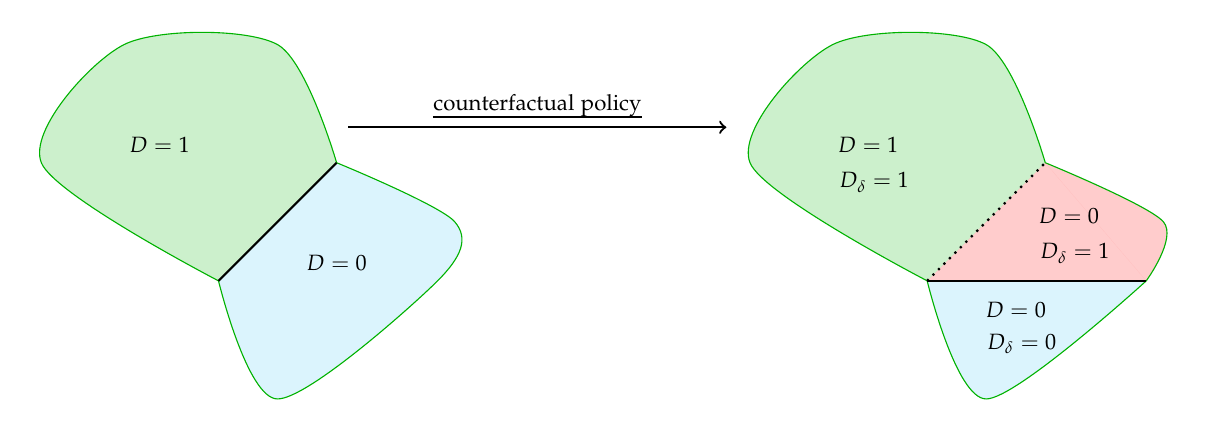
\begin{tikzpicture}[
    scale=1.5]

\draw [green, thin, fill=green, fill opacity=0.2] plot [smooth] coordinates {(0.5,2) (0,3) (-1.3,3) (-2,2) (-0.5,1)};
\draw [green, thin, fill=cyan!20, fill opacity=0.7] plot [smooth] coordinates {(-0.5,1) (0,0)  (1.355,1) (1.5, 1.5) (0.5,2) };



\draw [green, thin, fill=green, fill opacity=0.2] plot [smooth] coordinates {(6.5,2) (6,3) (4.7,3) (4,2) (5.5,1)};
\draw [green, thin, fill=cyan!20, fill opacity=0.7] plot [smooth] coordinates {(5.5,1) (6,0) (7.355,1)};
\draw [green, fill=red, fill opacity=0.2] plot [smooth] coordinates {(7.355,1) (7.5, 1.5) (6.5,2) };
\fill[fill=red, fill opacity=0.2] (6.5,2)--(7.355,1)--(5.5,1);



 \draw [->, thick] (0.6,2.3)-- (3.8,2.3);
\node [anchor=south] at (2.2,2.3) {\footnotesize\emph{counterfactual policy}};


 \draw [solid, thick] (-0.5,1)-- (0.5,2);
      \node [anchor=north] at (-1,2.3) {\footnotesize$D=1$};

        \node [anchor=north]  at (0.5,1.3) {\footnotesize$D=0$};
        
         \draw [dotted, thick] (5.5,1)-- (6.5,2);
         \draw [solid, thick] (5.5,1)-- (7.355,1);
      \node [anchor=north] at (5,2.3) {\footnotesize$D=1$};
        \node [anchor=north] at (5.05,2) {\footnotesize$D_\delta=1$};
            \node [anchor=north] at (6.7,1.7) {\footnotesize$D=0$};
                        \node [anchor=north] at (6.75,1.4) {\footnotesize$D_\delta=1$};

        \node [anchor=north]  at (6.25,0.9) {\footnotesize$D=0$};
                \node [anchor=north]  at (6.3,0.63) {\footnotesize$D_\delta=0$};


     
\end{tikzpicture}
\caption{\emph{A counterfactual policy where $D_\delta-D\geq 0$.}}
\label{figure_introduction}
\end{figure}


\begin{assumption}[Counterfactual Policies]\label{assumption_policy}
The collection of policies $\mathcal D$ satisfies
\begin{enumerate}
\item $\Pr(D_\delta=1)=p+\delta$ for $\delta\in[0,1-p)$ and $D_\delta\in\mathcal D$;
\item Monotonicity: $D_\delta-D\geq 0$;
%\item The counterfactual outcomes $Y_{D_\delta}$ are continuous with positive density on their support $\mathcal Y$. \textcolor{red}{PUT THIS IN TERMS OF PRIMITIVES. THAT WOULD BE BETTER ACTUALLY.}
\end{enumerate}
\end{assumption}

The monotonicity assumption $D_\delta-D\geq 0$ is mainly for expositional simplicity. We can do without this assumption, but we need to make some minor changes to our approach. However, there is also a practical purpose. In a context where $D$ is union status, and $D=1$ denotes unionized individuals, Assumption \ref{assumption_policy} requires that we increase the unionization rate by unionizing previously nonunionized workers. It would probably be hard to simultaneously unionize and deunionize different workers.

Another way to look at the monotonicity assumption is by inspecting the joint distribution of $D$ and $D_\delta$ it induces:
\begin{equation*}
\centering
\begin{tabular}{l|*{2}{c}r}
              & $D_{\delta }=0$ & $D_{\delta }=1$ \\
\hline
$D=0$ & $1-p-\delta$& $\delta$ \\
$D=1$            & $0$ &  $p$ \\
\end{tabular}
\end{equation*}

In other words, Assumption \ref{assumption_policy} rules out the presence of \emph{newly untreated} individuals. Also, in the limit, when $\delta=0$, we return to the original distribution of individuals. We will evaluate the effect of a counterfactual policy with two parameters: the global and the marginal effects. Let $F_Y^{-1}(\tau)$ and $F_{Y_{D_\delta}}^{-1}(\tau)$ denote the $\tau$-quantiles of $Y$ and $Y_{D_\delta}$ respectively.
\begin{definition}[Global and Marginal Effects]
For a given collection of policies $\mathcal D$, the unconditional global effect at the $\tau$-quantile of $D_\delta\in\mathcal D$ is
\begin{align*}
G_{\tau, D_\delta}&:=F_{Y_{D_\delta}}^{-1}(\tau)-F_{Y}^{-1}(\tau),
\end{align*}
and the unconditional marginal effect at the $\tau$-quantile is
\begin{equation*}
M_{\tau,\mathcal D}:=\lim_{\delta\to 0}\frac{F_{Y_{D_\delta}}^{-1}(\tau)-F_{Y}^{-1}(\tau)}{\delta}
\end{equation*}
whenever this limit exists.
\end{definition}

The global effect $G_{\tau, D_\delta}$ is the comparison of quantiles of the counterfactual distribution vs. the observed distribution for a fixed policy $D_\delta$. Naturally, for a collection $\mathcal D$, we have a corresponding collection on global effects. The marginal effect $M_{\tau,\mathcal D}$ can be interpreted as an ordinary derivative: for small $\delta$, it provides an approximation to the direction of the change in a given $\tau$-quantile.

\begin{remark}[\cite{Rothe2012}]
\cite{Rothe2012} also studies the global and marginal effects but under a different identifying assumption, namely a form of conditional exogeneity. This assumption also yields an identified set. Let the outcome be $Y=h(D,X,U)$. For uniformly distributed random variables $\tilde U_1$ and $\tilde U_2$, the outcome can be represented as $Y=h(Q_D(\tilde U_1),Q_X(\tilde U_2),U)$ where $Q_D$ and $Q_X$ are the quantile functions. Then $Q_D$ is changed to another quantile function $Q_D^*$, generating a counterfactual distribution, which is identified when $\tilde U_1\perp U\| X$ and $D$ is continuous. When $D$ is discrete, $\tilde U_1$ is not uniquely determined, so that a range of possible counterfactual distributions is possible resulting in partial identification.
\end{remark}


\begin{remark}[\cite{Firpo2009}]
The marginal effect $M_{\tau,\mathcal D}$ was originally studied by \cite{Firpo2009}. Instead of Assumption \ref{assumption_policy}, \cite{Firpo2009} assume a form of distributional invariance: $F_{Y_{D_\delta}|D_\delta=d}=F_{Y|D=d}$ and obtain point identification. See the proof to Corollary 3 of the working paper version \cite{Firpo2007}. When both $D$ and $D_\delta$ are independent of $U$ and $X$, then distributional invariance will be satisfied. In this particular case, a policy maker can randomize $D_{\delta}$  so that for a given $\delta$, a fraction $p+\delta$ of individuals is randomly assigned to treatment. However, if we allow for $D$ to be endogenous, and if, as is usually the case, the structural form of endogeneity is unknown, then it may be impossible for the policy maker to design a sequence $\mathcal D$, such that for every $D_\delta\in\mathcal D$, $F_{Y_{D_\delta}|D_\delta=d}$ ``matches'' $F_{Y|D=d}$. From the point of view of the policy maker, this is a significant restriction on the types of counterfactual policies they can consider.
\end{remark}

\begin{remark}[Policy Relevant Treatment Effect]
\cite{heckman_prte, Heckman2005} and \cite{Carneiro2010,Carneiro2011} investigate the effect on the unconditional mean of the outcome. Using our notation, the Policy Relevant Treatment Effect (PRTE) of \cite{heckman_prte, Heckman2005} is 
\begin{equation*}
\text{\textrm{PRTE}}_{D_\delta }=\frac{E(Y_{D_\delta })-E(Y)}{\delta}
\end{equation*}%
and taking the limit $\delta \rightarrow 0$ yields the Marginal PRTE (MPRTE) of \cite{Carneiro2010,Carneiro2011}:%
\begin{equation*}
\mathrm{MPRTE_\mathcal D}=\lim_{\delta \rightarrow 0}\text{\textrm{PRTE}}_{\delta }.
\end{equation*}
\cite{yixiao2020} show how to generalize the MPRTE to cover the case of \cite{Firpo2009} as well.
\end{remark}




The next task is to define \emph{who} are the \emph{newly treated} individuals, that is, how does $D_\delta$ determine who receives treatment among the individuals whose $D=0$? In this paper we will focus on two types of policies: a policy that simply chooses individuals whose $D=0$ at random and assigns them to $D_\delta=1$, and a policy that chooses individuals based on a user-specified criterion. We will refer to these two types of policies as \emph{randomized policy} and \emph{non-randomized policy} respectively. %A randomized policy might be more in line with a \textcolor{red}{TAKE THIS OUT ACTUALLY} concept of fairness: everyone in the untreated group gets an equal chance of being treated. A non-randomized policy, in contrast, might be more in line with a situation where the policy maker has a particular loss function they are trying to optimize. 

\begin{example}[Randomized policy]\label{example_rand_policy}
A randomized policy satisfies: for any $\delta\in[0,1-p)$
\begin{align*}
D_\delta = 
     \begin{cases}
       1 &\quad\text{if }D=1\\
        0 \text{ or }1 &\quad\text{if }D=0\\
     \end{cases}
\end{align*}
and the \emph{newly treated} are selected at random. Using the conditional independence notation\footnote{\cite{Dawid1979} writes $X\perp Y\|Z$ to denote that $X$ and $Y$ are independent conditional on $Z=z$ for any $z$. Here, we require independence to hold conditionally only on $D=0$.} we write $D_\delta\perp Y(1), Y(0)\|D=0$: 
\begin{align}\label{eqn_random_cia}
Pr(D_\delta=1|D=0)=\Pr(D_\delta=1|D=0, Y(1), Y(0))=\frac{\delta}{1-p}.
\end{align}
\end{example}



\begin{example}[Non-randomized policy]\label{example_non_rand_policy}
An example of a non-randomized policy is the following: for any $\delta\in[0,1-p)$
\begin{align}\label{eqn_non_random}
D_\delta = 
     \begin{cases}
       1 &\quad\text{if }D=1\\
        1 &\quad\text{if }D=0 \text{ and }Z\le F^{-1}_{Z|D=0}\left(\frac{\delta}{1-p}\right)\\
      0 &\quad\text{otherwise}\\
     \end{cases}
\end{align}
for some observable random variable $Z$. In this case, the individuals in the group $\left\{D=0\right\}$ whose $Z$ is less than the $\frac{\delta}{1-p}$-quantile of this group are shifted to $D_\delta=1$. This rule guarantees that, in expectation, a proportion $\delta$ of individuals is shifted.
\end{example}

For a collection of policies $\mathcal D$ that satisfies Assumptions \ref{assumption_policy}, the counterfactual distribution $F_{Y_{D_\delta}}(y)$ can be decomposed as
\begin{align}\label{count_dist_dec}
F_{Y_{D_\delta}}(y) &= pF_{Y|D=1}(y)  + (1-p-\delta) F_{Y|D_\delta=0}(y)  +\delta F_{Y(1)|D=0,D_\delta=1}(y)
\end{align}
for each $D_\delta$. Here, $F_{Y(1)|D=0,D_\delta=1}(y)$ corresponds to the distribution of the \emph{newly treated}. This distribution cannot be identified from the data because it requires observing $Y(1)$ for a subpopulation for which we only observe their $Y(0)$. Consequently, $F_{Y_{D_\delta}}(y)$ is not identified either. The goal is to bound the quantiles of $F_{Y_{D_\delta}}(y)$. To that end, we make the following regularity assumptions.

\begin{assumption}[Regularity Assumptions]\label{assumption_regularity}

\begin{enumerate}
\item\label{assumption_yd_regular} For $d=0,1$, $F_{Y|D=d,X=x}(y)$ is continuous and strictly increasing for all $y$ such that $0<F_{Y|D=d,X=x}(y)<1$, and for all $x\in\mathcal X$.
\item\label{assumption_yd_regular_2} For every $D_\delta\in\mathcal D$, $F_{Y|D_\delta=0}(y)$  is continuous and strictly increasing for all $y$ such that $0<F_{Y|D_\delta=0}(y)<1$.
\item For every $D_\delta\in\mathcal D$, $F_{Y(1)|D=0,D_\delta=1}(y)$  is continuous and strictly increasing for all $y$ such that $0<F_{Y(1)|D=0,D_\delta=1}(y)<1$.
%\item The support of $X$ is finite and is denoted by $\mathcal X$.
\item\label{assumption_x_support} For every $D_\delta\in\mathcal D$, the support of $X$ conditional on $D=0$ and $D_\delta=1$ is included in the support of $X$ conditional on $D=1$.
\end{enumerate}
\end{assumption}

%\textcolor{red}{I CHANGED ASSUMPTION 2.1. MAKE SURE IT DOES NOT INTERFERE WITH OTHERS.....}

The next assumption is our main working assumption to obtain the bounds on the quantiles of $F_{Y_{D_\delta}}(y)$.
\begin{assumption}[KS-distance]\label{assumption_ks_distance}
For a given $D_\delta\in\mathcal D$, there exists a known $c\in[0,1]$ such that
\begin{align}\label{eq:ks_distance}
c:=\sup_{y\in\mathbb R}\left |F_{Y(1)|D=0,D_\delta=1}(y)-\int_{\mathcal X}F_{Y|D=1,X=x}(y)dF_{X|D=0,D_\delta=1}(x)\right |.
\end{align}
\end{assumption}



We refer to $c$ as the \emph{policy selection bias}. The idea is that in the absence of policy selection bias, \emph{i.e.}, $c=0$, we can recover $F_{Y(1)|D=0,D_\delta=1}(y)$ by matching \emph{already} unionized individuals with \emph{newly} unionized individuals and integrating against the characteristics of the \emph{newly} unionized individuals, using $F_{X|D=0,D_\delta=1}(x)$. This is akin to a \textit{joint} unconfoundedness assumption: $D\perp Y(1)\| X$ \textit{and} $D_\delta\perp Y(1)\| X$.\footnote{If $D, D_\delta\perp Y(1)\| X$, then
\begin{align*}
F_{Y|D=1, X=x}(y)  = F_{Y(1)|D=0,D_\delta = 1, X=x}(y) 
\end{align*}
so that integrating against $F_{X|D=0,D_\delta=1}(x)$ yields $F_{Y(1)|D=0,D_\delta=1}(y) $.} By allowing $c$ to be non-zero, we are relaxing this particular type of conditional independence assumption (\cite{Masten2018}). Here, Assumption \ref{assumption_regularity}.\ref{assumption_x_support} becomes relevant.
\cite{Kline2013} also use the Kolmogorov-Smirnov distance to bound the quantiles of the outcome when data might not be missing at random.

%\textbf{Here I could show that the bounds hold pointwise for every $\delta$. That is the bounds are a collection of bounds that depend on $\mathcal D$.}

\begin{remark}
For now we take $c$ as known. In the next section it will be the quantity on which will be base the sensitivity analysis.
\end{remark}

\begin{theorem}[Bounds on the Global Effect]\label{thm_bounds_global}
If a policy $D_\delta$ satisfies assumptions \ref{assumption_policy}, \ref{assumption_regularity}, and \ref{assumption_ks_distance}, then for $\tau\in(\delta,1-\delta)$
\begin{align*}
\max\left\{\tilde F_A^{-1}(\tau-\delta) ,F_A^{-1}(\tau-\delta c)\right\} - F_{Y}^{-1}(\tau) \leq G_{\tau, D_\delta}\leq \min\left\{\tilde F_A^{-1}(\tau) ,F_A^{-1}(\tau+\delta c)\right\}-F_{Y}^{-1}(\tau)
\end{align*}
where $\tilde F_A(y):= p F_{Y|D=1}(y)  + (1-p-\delta) F_{Y|D_\delta=0}(y),$ and %$F_A(y):=\tilde F_A(y)  +\delta  \int_{\mathcal X}F_{Y|D=1,X=x}(y)dF_{X|D=0,D_\delta=1}(x).$
%\begin{align*}
%\tilde F_A(y)&:= p F_{Y|D=1}(y)  + (1-p-\delta) F_{Y|D_\delta=0}(y),\\
%\end{align*}
%and
\begin{align*}
F_A(y)&:=\tilde F_A(y)  +\delta  \int_{\mathcal X}F_{Y|D=1,X=x}(y)dF_{X|D=0,D_\delta=1}(x).
\end{align*}
These bounds are sharp.
\end{theorem}



\begin{remark}
When $c=0$, $G_{\tau, D_\delta}$ is point identified because the counterfactual distribution in \eqref{count_dist_dec} becomes $F_A(y)$, which is identified. We refer to $F_A(y)$ as the apparent distribution, hence the subscript $A$, because it is the distribution that ``appears'' to be the counterfactual distribution. Naturally, for $c=0$, we have that the lower and upper bound are identical, and equal to $F_A^{-1}(\tau)$.\footnote{\label{footnote}
For $c=0$, the upper bound is $F_A^{-1}(\tau)$ because $F_A^{-1}(\tau)\leq \tilde F_A^{-1}(\tau) $. For the lower bound we need to show that $\max\left\{\tilde F_A^{-1}(\tau-\delta),F_A^{-1}(\tau)\right\}=F_A^{-1}(\tau)$. Note that $\tilde F_A^{-1}(\tau-\delta)$ satifies:
\begin{align*}
p F_{Y|D=1}(\tilde F_A^{-1}(\tau-\delta))  + (1-p-\delta) F_{Y|D_\delta=0}(\tilde F_A^{-1}(\tau-\delta)) = \tau-\delta
\end{align*}
On the other hand, $F_A^{-1}(\tau)$ when $c=0$ satisfies
\begin{align*}
pF_{Y|D=1}(F_A^{-1}(\tau))  + (1-p-\delta) F_{Y|D_\delta=0}(F_A^{-1}(\tau))  +\delta  \int_{\mathcal X}F_{Y|D=1,X=x}(F_A^{-1}(\tau))dF_{X|D=0,D_\delta=1}(x)=\tau
\end{align*} 
Comparing these two expression, we obtain
\begin{align*}
p F_{Y|D=1}(\tilde F_A^{-1}(\tau-\delta))  + (1-p-\delta) F_{Y|D_\delta=0}(\tilde F_A^{-1}(\tau-\delta)) \leq 
pF_{Y|D=1}(F_A^{-1}(\tau))  + (1-p-\delta) F_{Y|D_\delta=0}(F_A^{-1}(\tau))  
\end{align*}
which implies that we must have $\tilde F_A^{-1}(\tau-\delta)\leq F_A^{-1}(\tau)$. 
} Thus, for $c=0$, $G_{\tau, D_\delta}= F_A^{-1}(\tau)-F_{Y}^{-1}(\tau)$.
\end{remark}

\begin{remark}
By construction, we have that $\tilde F_A(y)\leq F_A(y)$, which implies, for $\tau\in(\delta,1-\delta)$, that $ F_A^{-1}(\tau)\leq \tilde F_A^{-1}(\tau)$. Therefore, whether $F_A$ or $\tilde F_A$ bounds the global effect depends on $\tau$, $\delta$, and $c$. In other words, the $\min$ and $\max$ are not redundant.
\end{remark}


\begin{remark}
The bounds are sharp in the sense that for any possible value of the global effect within the bounds, there is a corresponding newly treated distribution $F_{Y(1)|D=0,D_\delta=1}(y)$ which delivers that same global effect.
\end{remark}

\begin{remark}\label{remark_tau}
The rage of $\tau$ is restricted to $(\delta,1-\delta)$ in order to ensure that $c$ to plays a role in the bounds. For $\tau$ outside this range, the bounds might not depend on $c$, if $c$ is close enough to 1.
\end{remark}

Before we attempt to bound the marginal effect, we will first investigate the issue of existence. To that end, we introduce the following assumption.
\begin{assumption}[Limiting Distributions]\label{assumption_limit_distribution}
 For a given sequence of policies $\mathcal D$, the following maps exist and are continuous on $y\in\mathbb R$:
 \begin{align*}
y\mapsto \frac{\partial F_{Y|D_\delta=0}(y)}{\partial \delta}\bigg|_{\delta=0}:= \lim_{\delta\to0} \frac{F_{Y|D_\delta=0}(y)-F_{Y|D=0}(y)}{\delta}
  \end{align*}
and
   \begin{align*}
y\mapsto   F_{Y(1)|\partial D}(y):=\lim_{\delta\to0}F_{Y(1)|D=0,D_\delta=1}(y).
  \end{align*}
  Moreover, convergence takes place uniformly:
  \begin{align*}
\lim_{\delta\to0}\sup_{y\in\mathbb R} \left|\frac{F_{Y|D_\delta=0}(y)-F_{Y|D=0}(y)}{\delta}-\frac{\partial F_{Y|D_\delta=0}(y)}{\partial \delta}\bigg|_{\delta=0} \right|=0,
\end{align*}
and
  \begin{align*}
\lim_{\delta\to0}\sup_{y\in\mathbb R} \left|F_{Y(1)|D=0,D_\delta=1}(y) - F_{Y(1)|\partial D}(y) \right| =0.
\end{align*}
  
  \end{assumption}

\begin{theorem}[Existence of Marginal Effect]\label{theorem_existence}
Let $\mathcal D$ be a sequence of policies such that Assumptions \ref{assumption_policy}, \ref{assumption_regularity}, and \ref{assumption_limit_distribution} hold. If $f_Y(F_Y^{-1}(\tau))>0$, then $M_{\tau,\mathcal D}$ exists and is given by
\begin{equation*}
M_{\tau,\mathcal D}=-\frac{\dot F_{Y,\mathcal D}(F_Y^{-1}(\tau))}{f_Y(F_Y^{-1}(\tau))}.
\end{equation*}
where $\dot F_{Y,\mathcal D}(y)$ satisfies
\begin{align*}
\lim_{\delta \downarrow 0}\sup_{y\in\mathbb R} \left|\frac{F_{Y_{D_\delta}}(y)-F_{Y}(y)}{\delta}-\dot F_{Y,\mathcal D}(y)\right|=0.
\end{align*}
\end{theorem}


The conditions and the proof of Theorem \ref{theorem_existence} come from viewing the marginal effect as a Hadamard derivative. Inspection of \eqref{count_dist_dec} shows that the assumptions of the theorem ensure that $\lim_{\delta\to 0}F_{Y_{D_\delta}}=F_Y$. That is, in the limit, the sequence of policies lead to the observed distribution of $Y$. To better understand the smoothness conditions imposed by Assumption \ref{assumption_limit_distribution} we provide an example and a counterexample.



\begin{example}\label{example_existence_of_marg}
Suppose that $D=\mathds 1\left\{ V\geq 0 \right\}$ for $V$ continuously distributed around 0. For a sequence $\delta\downarrow 0$, consider $D_\delta=\mathds 1\left\{ V\geq F_V^{-1}(F_V(0)-\delta) \right\}$. Then, for $p:=\Pr(D=1)$, we have that $\Pr(D_\delta=1)=p+\delta$.
Under mild conditions
\begin{align*}
\lim_{\delta\to 0}\frac{F_{Y|D_\delta=0}(y)-F_{Y|D=0}(y)}{\delta}=-\left(\frac{1}{f_V(0)}+\frac{1}{p}\right)F_{Y|D=0}(y)
\end{align*}
and 
\begin{align*}
\lim_{\delta\to0} F_{Y(1)|D=0,D_\delta=1}(y) = F_{Y(1)|V=0}(y)
\end{align*}
We can interpret $V=0$ as those individuals who are indifferent with respect to treatment. That is why we denote them with $\partial D$. See the appendix for detailed calculations. 

For a counterexample, consider instead $D_\delta=\mathds 1\left\{ V\leq F_V^{-1}(F_V(0)+\delta) \right\}$,  where the inequality sign is reversed. Here, $\Pr(D_\delta=1)=p+\delta$ provided $V$ is symmetric around 0: $F_V(0)=1-F_V(0)$. However,
\begin{align*}
F_{Y|D_\delta=0}(y)= \Pr(Y\leq y| V\geq F_V^{-1}(F_V(0)+\delta)) \to \Pr(Y\leq y| V\geq 0)  = F_{Y|D=1}(y).
\end{align*}
which contradicts the existence of the derivative $\frac{\partial F_{Y|D_\delta=0}(y)}{\partial \delta}\bigg|_{\delta=0}$ required in Assumption \ref{assumption_limit_distribution}.
\end{example}

To provide sharp bounds on the marginal effect we need the following assumption.
\begin{assumption}[More Limiting Distributions]\label{assumption_indifference}
 For a given sequence of policies $\mathcal D$, 
 \begin{enumerate}
 \item $\delta\mapsto F_{Y|D_{\delta}}(y)$ is differentiable at $\delta=0$ for every $y\in\mathbb R$.
 \item $\delta \mapsto F_{X| D=0, D_{\delta}=1}(x)$ is differentiable at $\delta=0$ for every $x\in\mathcal X$. Moreover, we denote $ F_{X|\partial D}(x):=     \lim_{\delta\downarrow0} F_{X| D=0, D_{\delta}=1}(x).$
\end{enumerate}
  \end{assumption}
Here, $F_{X|\partial D}(x)$ can be seen as the observable characteristics of the those individuals who are ``indifferent'' to treatment. Indeed, for the case of Example \ref{example_existence_of_marg}, we have $F_{X|\partial D}(x)=F_{X|V}(x|0)$.



\begin{theorem}[Bounds on the Marginal Effect]\label{thm_bounds_marginal}
If Assumptions \ref{assumption_policy}, \ref{assumption_regularity}, \ref{assumption_limit_distribution}, and \ref{assumption_indifference} hold, Assumption \ref{assumption_ks_distance} holds for all $\delta$ in a neighborhood of 0, and $F_{X|\partial D}$ is known, then, for $\tau\in(0,1)$, 
\begin{align*}
\theta_{L,M} \leq M_{\tau, \mathcal D} \leq \theta_{U,M}
\end{align*}
where
\begin{align*}
\theta_{L,M}:=\max\left\{\frac{F_{Y|D=0}(F^{-1}_{Y}(\tau))-1}{f_{Y}( F^{-1}_{Y}(\tau))} ,\frac{F_{Y|D=0}(F^{-1}_{Y}(\tau))-\int_{\mathcal X}F_{Y|D=1,X=x}(F^{-1}_{Y}(\tau))dF_{X|\partial D}(x)-c}{f_{Y}( F^{-1}_{Y}(\tau))}  \right\},
\end{align*}
and
\begin{align*}
\theta_{U,M}:=\min\left\{\frac{F_{Y|D=0}(F^{-1}_{Y}(\tau))}{f_{Y}( F^{-1}_{Y}(\tau))},\frac{F_{Y|D=0}(F^{-1}_{Y}(\tau))-\int_{\mathcal X}F_{Y|D=1,X=x}(F^{-1}_{Y}(\tau))dF_{X|\partial D}(x)+c}{f_{Y}( F^{-1}_{Y}(\tau))}\right\}.
\end{align*}
These bounds are sharp. 
\end{theorem}

\begin{remark}
The bounds for $M_{\tau, \mathcal D}$ require knowledge of $F_{X|\partial D}(x)$, \emph{i.e.}, the covariates for the individuals along the margin of indifference. One option is to set $F_{X|\partial D}(x)=F_{X| D=1}(x)$: marginal individuals have the (observable) characteristics of those with $D=1$. In this case, covariates no longer play a role in the bounds because
\begin{align*}
\int_{\mathcal X}F_{Y|D=1,X=x}(F^{-1}_{Y}(\tau))dF_{X|\partial D}(x)=\int_{\mathcal X}F_{Y|D=1,X=x}(F^{-1}_{Y}(\tau))dF_{X| D=1}(x)=\tau.
\end{align*}
A more general approach is to consider, for some $\alpha\in[0,1]$
\begin{align}\label{convex_covariates}
F_{X|\partial D}(x)=\alpha F_{X| D=1}(x) + (1-\alpha)F_{X| D=0}(x).
\end{align}
It must be kept in mind that any choice of $F_{X|\partial D}(x)$ entails a risk of misspecification. This makes the problem of bounding the marginal effect much harder.
\end{remark}


\begin{remark}
If we set $c=0$, and if Assumption \ref{assumption_ks_distance} holds for all $\delta$ in a neighborhood of 0, upon taking the limit in \eqref{eq:ks_distance} we obtain
\begin{align*}
F_{Y(1)|\partial D}(y)=\int_{\mathcal X}F_{Y|D=1,X=x}(y)dF_{X|\partial D}(x)
\end{align*}
for all $y\in\mathbb R$. This opens a number of ways to point identify the marginal effect. For example, we could require either $F_{Y(1)|\partial D}(y)=F_{Y| D=1}(y)$ or $F_{X|\partial D}(x)=F_{X| D=1}(x)$. In either case, we obtain
\begin{align*}
M_{\tau, \mathcal D} = \frac{F_{Y|D=0}(F^{-1}_{Y}(\tau))-F_{Y|D=1}(F^{-1}_{Y}(\tau))}{f_{Y}( F^{-1}_{Y}(\tau))},
\end{align*}
which is precisely the estimand of \cite{Firpo2009}. We could use \eqref{convex_covariates} for a given $\alpha$ to obtain yet a different value for the marginal effect.
\end{remark}

\begin{remark}
The bounds are sharp in the sense that for any possible value of the marginal effect within the bounds, there is a corresponding sequence of newly treated distribution $F_{Y(1)|D=0,D_\delta=1}(y)$ which delivers that same marginal effect.
\end{remark}



\section{Quantile Breakdown Frontier}

The quantile breakdown frontier is a curve that allows to perform to a sensitivity analysis with respect to $c$, the policy selection bias. Suppose we are interested in a target conclusion $G_{\tau,D_\delta}\geq g_{\tau,L} $ for some $g_{\tau,L}$. If the conclusion does not hold under point identification, \textit{i.e.} when $c=0$, then there is no point in performing a sensitivity analysis. On the other hand, if the conclusion does hold under point identification, we would like to know the maximum amount of such that $c$ such that the conclusion continues to hold. This is the sensitivity analysis. 
The quantile breakdown frontier for the global effect tackles both of these issues. The frontier is the map
\begin{align}\label{qbf_def}
\tau\mapsto c_{\tau,L}= \frac{\tau -F_A\left ( F_{Y}^{-1}(\tau)+ g_{\tau,L} \right )}{\delta}
\end{align}
for $\tau\in(\delta,1-\delta)$.\footnote{We can also look at conclusions of the type $G_{\tau,D_\delta}\leq g_{\tau,U}$. In this case, the quantile breakdown frontier is the map
\begin{align*}
\tau\mapsto c_{\tau,U}= \frac{F_A\left ( F_{Y}^{-1}(\tau)+ g_{\tau,U} \right )-\tau}{\delta}.
\end{align*}
%Two sided conclusions: $ g_{\tau,L}\leq G_{\tau,D_\delta}\leq  g_{\tau,U}$ can be handled by $\tau \mapsto c(\tau)=\min \left \{  c_{\tau,L}, c_{\tau,U} \right\}$.
} 
When $c_{\tau,L}<0$, the desired target conclusion does not hold. If $c_{\tau,L}>0,$ then for $c\leq  c_{\tau,L}$ then target conclusion holds under point identification. If $c> c_{\tau,L}>0$, then the target conclusion might not hold. In this sense, when $c_{\tau,L}>0,$ the frontier provides an amount of policy selection bias which is compatible with the conclusion.

The next lemma contains some properties of the quantile breakdown frontier.

\begin{lemma}\label{qbf_global_lemma}
Under the assumptions of Theorem \ref{thm_bounds_global}, the quantile breakdown frontier for $G_{\tau,D_\delta}$ defined in \eqref{qbf_def} satisfies the following: (i) if $\tau\mapsto g_{\tau,L}$ is continuous, then $\tau\mapsto c_{\tau,L}$ is continuous; (ii) if $c_{\tau,L}<0$, then the conclusion does not hold under point identification; (iii) if $c_{\tau,L}\geq 0$, then for any $c\geq 0$ such that $c\leq  c_{\tau,L}$, the conclusion holds, and for $c> c_{\tau,L}$ the conclusion might not hold; and (iv) if $\tilde F_A^{-1}(\tau-\delta)\geq F_A^{-1}(\tau-\delta c_{\tau,L})$, then the conclusion holds for any $c\in[0,1]$.
\end{lemma}


Part $(i)$ of the lemma puts a restriction on the types of conclusion by requiring continuity of the family of target conclusions. This is no essential, but illustrates the fact that the smoothness of the frontier depends, among other things, on the conclusions. For notational simplicity, later on we assume $g_{\tau,L}\equiv g$. Part $(iv)$ addresses a potential ``conservadurism'' in the breakdown analysis. This stems from the fact there is a possibility that the lower bound for the global effect does not depend on $c$. In the notation of Theorem \ref{thm_bounds_global}, this means that we cannot rule out
\begin{align*}
\max\left\{\tilde F_A^{-1}(\tau-\delta) ,F_A^{-1}(\tau-\delta c)\right\} = \tilde F_A^{-1}(\tau-\delta).
\end{align*}
This is related to part $(ii)$. Indeed, if the opposite is true, $\tilde F_A^{-1}(\tau-\delta)< F_A^{-1}(\tau-\delta c_{\tau,L})$, then we can modify the language of part $(ii)$
 to say that for $c> c_{\tau,L}$ the conclusion \textit{will} not hold. In the empirical application we estimate $\tilde F_A^{-1}(\tau-\delta)\geq F_A^{-1}(\tau-\delta c_{\tau,L})$ and we rule out this case. 



For the marginal effect we can construct the quantile breakdown frontier in a similar fashion. However, in order to avoid the presence of the density $f_Y$ in the denominator,\footnote{Avoiding $f_Y$ allows us to retain a $\sqrt n$-consistent estimator.} we focus on conclusions $M_{\tau,\mathcal D}\leq 0$.\footnote{The case $M_{\tau,\mathcal D}\geq 0$ can be dealt with in the same way after some minor modifications. It is therefore omitted.} Thus, instead of a collection of conclusions that may vary with $\tau$, here we have a common conclusion across $\tau$. Since the marginal effect is a derivative, this amounts to looking at conclusions of whether the global effect in a neighborhood of $\delta=0$ is increasing or decreasing as $\delta$ increases. The quantile breakdown frontier for the marginal effect is the map
\begin{align}\label{qbf_def_marg}
\tau\mapsto c_{\tau,U}^M= \int_{\mathcal X}F_{Y|D=1,X=x}(F^{-1}_{Y}(\tau))dF_{X|\partial D}(x)-F_{Y|D=0}(F^{-1}_{Y}(\tau)),
\end{align}
for $\tau\in (0,1)$. The next lemma is analogous to Lemma \ref{qbf_global_lemma}.

\begin{lemma}\label{qbf_marginal_lemma}
Under the assumptions of Theorem \ref{thm_bounds_marginal}, the quantile breakdown frontier for $M_{\tau,\mathcal D}$ defined as the map in \eqref{qbf_def_marg} satisfies the following: (i) $\tau\mapsto c_{\tau,U}^M$ is continuous; (ii) if $c_{\tau,U}^M<0$, then the conclusion does not hold under point identification; (iii) if $c_{\tau,U}^M\geq 0$, then for any $c\geq 0$ such that $c\leq  c_{\tau,U}^M$, the conclusion holds, and for $c> c_{\tau,U}^M$ the conclusion might not hold; and (iv) if $F_{Y|D=0}(F^{-1}_{Y}(\tau))\leq \int_{\mathcal X}F_{Y|D=1,X=x}(F^{-1}_{Y}(\tau))dF_{X|\partial D}(x)$, then the conclusion holds for any $c\in[0,1]$.
\end{lemma}

\begin{remark}
While the frontier for the global effect is valid for $\tau\in (\delta, 1-\delta)$, for the marginal effect it is valid for $\tau\in(0,1)$, provided that $Y$ has a bounded support. This difference arises because in the marginal effect we are taking the limit as $\delta\to 0$.
\end{remark}


\subsection{Bounds derived from the QBF}
Suppose that a policy maker choose a particular quantile $\tau^*$ and a target conclusion $g_{\tau^*,L}$. Then, provided that $c_{\tau^*,L}\in [0,1]$, we can obtain bounds on the global effect other quantiles $\tau\neq \tau^*$. The interpretation is that, as long as the policy selection bias satisfies $c\leq c_{\tau^*,L}$, the global effect will be bounded across quantiles by the bounds of Theorem \ref{thm_bounds_global} evaluated at $c_{\tau^*,L}$. In a sense, this allows us to extend the sensitivity analysis to other quantiles. That is for $\tau\in(\delta,1-\delta)$, we have
\begin{align}\label{eq:bounds_derived}
\max\left\{\tilde F_A^{-1}(\tau-\delta) ,F_A^{-1}(\tau-\delta c_{\tau^*,L})\right\} - F_{Y}^{-1}(\tau) \leq G_{\tau, D_\delta}\leq \min\left\{\tilde F_A^{-1}(\tau) ,F_A^{-1}(\tau+\delta c_{\tau^*,L})\right\}-F_{Y}^{-1}(\tau).
\end{align}








\section{Estimation and Inference}


We work in the space $\ell^{\infty}(\delta,1-\delta)$ of bounded real-valued functions defined on $(\delta,1-\delta)$. As usual, we endow this space with the supremum norm: $\|x\|_\infty:=\sup_{t\in(\delta,1-\delta)}|x(t)|$.\footnote{The reason we restrict the space to be $\ell^{\infty}(\delta,1-\delta)$ and not $\ell^{\infty}(0,1)$ is due to the fact that for a given $\delta$, we cannot reach quantiles below $\delta$ or above $1-\delta$. See Remark \ref{remark_tau} above.} In order to simplify notation, and ensure the continuity of the quantile breakdown frontier, we are going to focus on the case where the threshold is constant across $\tau$.

\begin{assumption}[Constant Threshold]\label{uniform_threshold}
For some scalar $g$, the threshold $g_{\tau,L}$ satisfies $g_{\tau,L}=g$ for any $\tau\in(\delta,1-\delta)$. 
\end{assumption}

This assumption can be relaxed at the expense of more complicated notation. However, we still require smoothness in the map $\tau\mapsto g_\tau.$ For the case of the quantile breakdown for the sign of the marginal effect, we will set $g=0$. 

\begin{assumption}[DGP]\label{dgp}
We observe an i.i.d. sample $\{ Y_i, D_i, X_i \}_{i=1}^n$, where the support of $X$ is finite.
\end{assumption}


\subsection{Global Effect}
To estimate $ c_{\tau,L}$ given in \eqref{qbf_def} we need to specify two components: $(i)$ $\delta$, the increase in the treated proportion, and $(ii)$
$D_{i,\delta}$, the counterfactual treatment assignment, as in examples \ref{example_rand_policy} and \ref{example_non_rand_policy}. Once this has been done, 
we use sample analogs. The estimator of the quantile breakdown frontier for the global effect is
\begin{align}\label{qbf_estimation}
%\hat c_{\tau,L}= \max \left \{  \min \left \{ \frac{\hat F_A\left ( \hat F_{Y}^{-1}(\tau)+ g \right )-\tau}{\delta}, 1\right\},0 \right\}
\hat c_{\tau,L}= \frac{\tau - \hat F_A\left ( \hat F_{Y}^{-1}(\tau)+ g \right )}{\delta},
\end{align}
where $ \hat F_{Y}^{-1}(\tau)$ is the empirical $\tau$-quantile of $Y$: $\hat F_Y^{-1}(\tau) :=\inf \left\{ y:\hat F_Y(y)\geq \tau  \right\}$, and $\hat F_A(y)$ is the empirical counterpart of $F_A(y)$ given in Theorem \ref{thm_bounds_global}. Detailed expressions are provided in Appendix \ref{appendix_notation}. 
%Define 
%\begin{align*}
%\hat \theta(\tau)= \frac{\hat F_A\left ( \hat F_{Y}^{-1}(\tau)+ g \right )-\tau}{\delta}.
%\end{align*}
This is similar to a quantile-quantile transformation (see Exercise 4 in Chapter 3.9 in \cite{vandervaart1996}). We base our proof of the asymptotic distribution of $\sqrt n(\hat c_{\tau,L}-c_{\tau,L})$ on the proof of Lemma A.1 in \cite{Beare2019}.\footnote{\cite{Beare2019} also offer some interesting historical context for the result.} We view the map $\tau\mapsto\hat c_{\tau,L}$ as a random element of $\ell^{\infty}(\delta,1-\delta)$. In that case, we denote it simply by $\hat c_{L}.$ %When viewed as a process in $\ell^{\infty}(\delta,1-\delta)$, the quantile breakdown frontier is denoted by
% \begin{align*}
%c_{L}= \frac{\hat F_A\left ( \hat F_{Y}^{-1}(\cdot)+ g \right )-\cdot}{\delta}.
%\end{align*}

The main assumption is the following.
\begin{assumption}[Functional CLT]\label{brownian_bridge}
The following multivariate functional central limit theorem holds 
\begin{align*} 
\sqrt n\begin{pmatrix}
\hat F_{Y} - F_Y\\
\hat F_{A}-  F_{A} 
%\hat F_{Y|D=1}-  F_{Y|D=1} \\
%\hat F_{Y|D_\delta=0}-  F_{Y|D_\delta=0}\\
%\hat F_{Y|D=1,X=x} - F_{Y|D=1,X=x}\\
%\hat F_{X|D=0,D_\delta=1}(x) -F_{X|D=0,D_\delta=1}(x) 
%\hat p-p
\end{pmatrix} \rightsquigarrow \begin{pmatrix}
\mathbb G_Y\\ 
\mathbb G_{A}
%\mathbb G_{1} \\ \mathbb G_{0,\delta}\\ \mathbb G_{1,x} \\  \mathbb Z_x \\ \mathbb Z_p
\end{pmatrix},
\end{align*}
%where $ \mathbb G_Y$, $ \mathbb G_{1}$, $\mathbb G_{0,\delta}$, and $ \mathbb G_{1,x} $ are Brownian bridges in $\ell^{\infty}(\mathcal Y)$, $Z_x$ is a $\mathcal X$-dimensional normal random variable, and $\mathbb Z_p$ is a real-valued normal random variable. 
where $\mathbb G_Y$ and $\mathbb G_A$ are Brownian bridges in $\ell^{\infty}(\mathcal Y)$.
\end{assumption}

\begin{remark}
More primitive assumptions in terms of the CDFs that comprise $F_A$ can be stated that lead to Assumption \ref{brownian_bridge}. For brevity, we leave it as it is.
\end{remark}


The following assumption is needed to establish the Hadamard differentiable of different functions used in the construction of $\theta$.
\begin{assumption}[Conditions for Hadamard Differentiability]\label{ass_had_dif}
\item
\begin{enumerate}
\item \label{ass_f_y_quantiles}For some $\varepsilon>0$, $F_Y$ is continuously differentiable in $[F_Y^{-1}(\delta)-\varepsilon,F_Y^{-1}(1-\delta)+\varepsilon]\subset \mathcal Y$ with strictly positive derivative $f_Y$.
\item  \label{ass_f_a_uniform}$y\mapsto F_A(y)$ is differentiable, with uniformly continuous and bounded derivatives.
%The distribution functions $ F_{Y|D=0,D_\delta=0}(y)$ and $ F_{Y|D=1,D_\delta=1}(y)$ are differentiable, with uniformly continuous and bounded derivatives on their support $\mathcal Y$. 
\end{enumerate}
\end{assumption}

The first item in Assumption \ref{ass_had_dif} concerns the support $\mathcal Y$ and the smoothness of $F_Y$. It is used to guarantee the Hadamard differentiability of the quantile process $\tau\mapsto F_Y^{-1}(\tau)$ for $\tau\in(\delta,1-\delta)$. The second item ensures that $F_A(y)$ has a uniformly continuous and bounded derivative which we denote by $f_A(y)$. It is needed to establish the Hadamard differentiability of the composition map $(F_A,F_Y^{-1})\mapsto F_A\circ (F_Y^{-1}+g)$.\footnote{Section 3.9 in \cite{vandervaart1996} studies the Hadamard differentiability of composition maps.}

\begin{theorem}\label{dist_theta}
Under Assumptions \ref{uniform_threshold}, \ref{dgp}, \ref{brownian_bridge}, and \ref{ass_had_dif}
\begin{align*}
\sqrt n(\hat c_{L}- c_{L})\rightsquigarrow \frac{1}{\delta}\mathbb G_A\circ (F_Y^{-1}+g)-\frac{1}{\delta}f_A\circ (F_Y^{-1}+g) \frac{\mathbb G_Y\circ F_Y^{-1}}{f_Y\circ F_Y^{-1}},
%\sqrt n(\phi(\hat\theta)-\phi(\theta)&\rightsquigarrow  \phi'_{\theta}(\mathbb G_{\theta}),
\end{align*}
%where
 %\begin{align*}
%\phi'_\theta(\mathbb G_{\theta}) =
%\mathbb G_{\theta}\mathds{1}_{\left\{0< \theta< 1 \right\}} + \max(0,\mathbb G_{\theta})\mathds{1}_{\left\{\theta= 0 \right\}} + \min (0,\mathbb G_{\theta})\mathds{1}_{\left\{\theta= 1 \right\}},
%\end{align*}
%and 
 %\begin{align*}
%\mathbb G_\theta:=-\frac{1}{\delta}\mathbb G_A\circ (F_Y^{-1}+g)+\frac{1}{\delta}f_A\circ (F_Y^{-1}+g) \frac{\mathbb G_Y\circ F_Y^{-1}}{f_Y\circ F_Y^{-1}}
%\end{align*}
a tight Gaussian element in $\ell^{\infty}(\delta,1-\delta)$.
\end{theorem}

Instead of providing a closed form expression and a consistent estimator for the variance of the quantile breakdown frontier, we note that, by Theorem 23.9 in \cite{vandervaart2000}, the empirical bootstrap is valid. Confidence intervals can be constructed following the usual resampling scheme.

\subsection{Marginal Effect}


%For the marginal effect, instead of $\delta$ and $D_{i,\delta}$, we have to provide $\hat F_{X|\partial D}(x)$. \textcolor{red}{Talk a bit about this.} Using sample analogs we obtain the following estimator of \eqref{qbf_def_marg}
For the marginal effect, using sample analogs we obtain the following estimator of \eqref{qbf_def_marg}.
\begin{align}\label{qbf_estimation_marg}
%\hat c_{\tau}= \max \left \{   \min\left\{ \sum_ {x\in\mathcal X}\hat F_{Y|D=1,X=x}(\hat F^{-1}_{Y}(\tau))\hat p_{x|\partial D}-\hat F_{Y|D=0}(\hat F^{-1}_{Y}(\tau)),1\right\},0 \right\}
\hat c_{\tau,U}^M = \sum_ {x\in\mathcal X}\hat F_{Y|D=1,X=x}(\hat F^{-1}_{Y}(\tau))\hat p_{x|\partial D}-\hat F_{Y|D=0}(\hat F^{-1}_{Y}(\tau))
\end{align}
%where 
%\begin{align*}
%\hat F_{Y|D=0}(y) = \frac{\sum_{i=1}^n\mathds1\{Y_i\leq y\}(1-D_i)}{\sum_{i=1}^n((1-D_i))}.
%\end{align*}
%and
%\begin{align*}
%\sum_ {x\in\mathcal X}\hat F_{Y|D=1,X=x}(y)\hat p_{x|\partial D}= \sum_{x\in \mathcal X} \frac{\sum_{i=1}^n  \mathds 1 \left\{Y_i\leq y \right\}D_i  \mathds 1 \left\{X_i=x \right\} }{\sum_{i=1}^n  D_i  \mathds 1 \left\{X_i=x \right\}  }\hat p_{x|\partial D} 
%\end{align*}
Here, $\hat p_{x|\partial D}$ is the empirical counterpart of $\Pr(X=x|\partial D)$, which, as mentioned above, is the distribution of covariates for individuals at the margin of indifference. By Assumption \ref{assumption_indifference}, this is $ F_{X|\partial D}(x):=     \lim_{\delta\downarrow0} F_{X| D=0, D_{\delta}=1}(x).$ Following \eqref{convex_covariates}, for a \emph{user-supplied} $\alpha$, we take $F_{X|\partial D}(x)=\alpha F_{X| D=1}(x) + (1-\alpha)F_{X| D=0}(x).$ Thus, 
\begin{align*}
\hat p_{x|\partial D} =\alpha \hat F_{X| D=1}(x) + (1-\alpha)\hat F_{X| D=0}(x).
\end{align*}
Details are given in Appendix \ref{appendix_notation}. The main assumption is 
\begin{assumption}[Functional CLT]\label{brownian_bridge_marginal}
The following multivariate functional central limit theorem holds 
\begin{align*} 
\sqrt n\begin{pmatrix}
 \sum_ {x\in\mathcal X}\hat F_{Y|D=1,X=x} \hat p_{x|\partial D} - E[F_{Y|D=1,X}|\partial D]\\
\hat F_{Y|D=0}-F_{Y|D=0} \\
\end{pmatrix} \rightsquigarrow \begin{pmatrix}
\mathbb G_{\partial D}\\ \mathbb G_{0}
\end{pmatrix},
\end{align*}
where $ \mathbb G_{\partial D}$ and $\mathbb G_{0}$ are Brownian bridges in $\ell^{\infty}(\mathcal Y)$.
\end{assumption}
Here, $E[F_{Y|D=1,X}|\partial D]$ implicitly denotes the map $y\mapsto E[F_{Y|D=1,X}(y)|\partial D]$. That is, the expectation is taken with respect to $X$ using $ F_{X|\partial D}(x)$. By Assumption \ref{dgp}, this expectation is just a 
finite convex combination of the distribution functions $F_{Y|D=1,X=x}(y)$ 

\begin{remark}
More primitive conditions, in terms of $F_{Y|D=1,X=x}(y)$, $F_{X| D=0}(x)$, and $F_{X| D=1}$ can be given that result in Assumption \ref{brownian_bridge_marginal}. %However, we prefer the way it is stated for economy of space.
\end{remark}


The next assumption is needed to establish the Hadamard differentiability of the composition map, and the quantile process.

\begin{assumption}[Conditions for Hadamard Differentiability]\label{ass_had_dif_2}
\item
\begin{enumerate}
\item The distribution functions $ F_{Y|D=0}(y)$ and $ E[F_{Y|D=1,X}(y)|\partial D]$ are differentiable, with uniformly continuous and bounded derivatives on their support $\mathcal Y$. The derivatives are denoted by  $f_{Y|D=0}(y)$ and $E[f_{Y|D=1,X}(y)|\partial D]$ respectively.
\item The support $\mathcal Y$ is the compact set $[y_l,y_u]$.
\item $F_Y(y)$ is continuously differentiable on $\mathcal Y$ with strictly positive derivative $f_Y$.
\end{enumerate}
\end{assumption}

 %As in Theorem \ref{dist_theta}, define
%\begin{align*}
%\hat \theta_M(\tau)& :=  \sum_ {x\in\mathcal X}\hat F_{Y|D=1,X=x}(\hat F^{-1}_{Y}(\tau))\hat p_{x|\partial D}-\hat F_{Y|D=0}(\hat F^{-1}_{Y}(\tau)),\\
%\theta_M(\tau) &:= E[F_{Y|D=1,X}(F^{-1}_{Y}(\tau))|\partial D]- F_{Y|D=0}( F^{-1}_{Y}(\tau)).
%\end{align*}
%Therefore, $c_\tau= \max \left \{  \min \left \{  \theta_M(\tau), 1\right\},0 \right\}$.
The next theorem establishes the asymptotic distribution of $\hat c_{\tau,U}^M$ as a process in $\ell^{\infty}(0,1)$. In such a case, we denote the process simply by $\hat c_{U}^M$.

\begin{theorem}[Asymptotic Distribution of QBF for Marginal Effect]\label{qbf_marginal}
Under Assumptions \ref{dgp}, \ref{brownian_bridge_marginal} and \ref{ass_had_dif_2}
\begin{align*}
\sqrt n(\hat c_{U}^M- c_{U}^M)&\rightsquigarrow   \mathbb G_{\partial D,Y}- \mathbb G_{0,Y},
%\phi'_{\theta_M}(\mathbb G_{\theta_M}),
\end{align*}
%where
 %\begin{align*}
%\phi'_{\theta_M}(\mathbb G_{\theta_M}) =
%\mathbb G_{\theta_M}\mathds{1}_{\left\{0< \theta_M< 1 \right\}} + \max(0,\mathbb G_{\theta_M})\mathds{1}_{\left\{\theta_M= 0 \right\}} + \min %(0,\mathbb G_{\theta_M})\mathds{1}_{\left\{\theta_M= 1 \right\}}.
%\end{align*}
where 
\begin{align*}
\mathbb G_{\partial D,Y}&=\mathbb G_{\partial D}\circ F_Y^{-1}-E[f_{Y|D=1,X}|\partial D]\circ F_Y^{-1} \cdot \frac{\mathbb G_Y\circ F_Y^{-1}}{f_Y\circ F_Y^{-1}},\\
\mathbb G_{0,Y}&=\mathbb G_0\circ F_Y^{-1}-f_{Y|D=0}\circ F_Y^{-1} \cdot \frac{\mathbb G_Y\circ F_Y^{-1}}{f_Y\circ F_Y^{-1}}.
\end{align*}
\end{theorem}

As in the case of the quantile breakdown frontier for the global effect, the empirical bootstrap is valid and can be used to construct confidence intervals.




\subsection{Bounds derived from the QBF}
To estimate the bounds derived the from the QBF for the global effect, we use the sample counterpart of \eqref{eq:bounds_derived}. Besides the target conclusion $g$ for the global effect, we need to supply, a quantile level $\tau^*$ of interest. For 
$\tau\in(\delta,1-\delta)$, the estimator of the derived bounds is
\begin{align*}
\max\left\{\hat{\tilde F}_A^{-1}(\tau-\delta) ,\hat F_A^{-1}(\tau-\delta \hat {\tilde c}_{\tau^*,L})\right\} - \hat F_{Y}^{-1}(\tau) \leq G_{\tau, D_\delta}\leq \min\left\{\hat{\tilde F}_A^{-1}(\tau) ,\hat F_A^{-1}(\tau+\delta \hat {\tilde c}_{\tau^*,L})\right\}- \hat F_{Y}^{-1}(\tau),
\end{align*}
where 
%\begin{align}
%\tilde c_{\tau^*,L} =  \max \left \{  \min \left \{  c_{\tau^*,L}, 1\right\},0 \right\}.
%\end{align}
%and 
\begin{align}
\hat {\tilde c}_{\tau^*,L} =  \max \left \{  \min \left \{  \hat c_{\tau^*,L}, 1\right\},0 \right\}.
\end{align}
Here, $\hat c_{\tau^*,L}$ is the estimator given in \eqref{qbf_estimation} evaluated $\tau=\tau^*$.

The asymptotic distribution of the bounds is not Gaussian. Hence, by Corollary 3.1 in \cite{Fang2019}, the standard bootstrap will fail. This means that if we attempt to construct confidence intervals in the usual way by resampling, we will not obtain correct asymptotic coverage. An alternative is to use the numerical delta method of \cite{Hong2018}.



\section{Empirical application: What do unions do?}\label{section_empirical}

There is an extensive literature that studies unions and inequality. A recent contribution by \cite{Farber2020} contains a review of the literature. In our empirical application, in particular, we look at how unions affect the distribution of wages for \emph{all} workers. Unions can have a variety of effects on the distribution of wages. As argued by \cite{Freeman1980}, unions can raise the wages of unionized workers relative to non-unionized workers, possibly through more bargaining power. So, if higher paid workers unionize, the dispersion of wages can increase, but if lower paid workers unionize, the dispersion of wages can decrease. Furthermore, within a given industry, the union can reduce the dispersion of wages by standardizing the wages. This will impact the distribution of wages more or less depending on the size of the industry and the wages it pays. 

A key difficulty in identifying the causal effect of unions on wages is that selection into unions is non-random. Hence, any measurement of the union premium--the difference in wages between similar union and nonunion workers--will be biased for the causal effect. Indeed, this has been a long standing concern of labor economists.\footnote{Indeed, the opening words of \cite{Card1996} are: \begin{quotation}
\emph{Despite a large and sophisticated literature there is still substantial disagreement over the extent to which differences in the structure of wages between union and nonunion workers represent an effect of trade unions, rather than a consequence of the nonrandom selection of unionized workers.}
\end{quotation}} With respect to selection into unions, \cite{Card1996} argues that unionized workers with low observed skills, tend to have high unobserved skills. The reverse happens with high skilled unionized workers: they tend to have low unobservable skills. Due to this selection bias, it might be impossible for a policy maker to devise a policy where the \emph{newly} unionized workers are selected in a way such that they are drawn from the distribution of the \emph{already} unionized workers.

Using the techniques developed in this paper, we are going to consider the effect of both globally and marginally expanding union coverage. We will explicitly allow for non-random selection into unions. %Moreover, as opposed to \cite{Firpo2009}, we will not assume distributional invariance: the distribution of the \emph{newly} unionized workers can be different from the distribution of the \emph{already} unionized workers. That is, we do not use any imputation method to impute the union premium of the newly unionized workers.
This allows for the \emph{newly} unionized and \emph{already} unionized workers to be drawn from different distributions. We do not use any imputation method to impute the union premium of the newly unionized workers.

Following \cite{Freeman1980}, \cite{Card2001} and \cite{Card2004} we consider a two sector economy. Each worker has a well-defined pair of potential (log) wages: $Y_i(1)$ for the unionized sector and $Y_i(0)$ for the nonunionized sector. Under Assumption \ref{assumption_policy}, and for any policy $D_\delta$, we have the following classification of individuals:
\begin{equation*}
\centering
\begin{tabular}{l|*{2}{c}r}
              & $D_{\delta }=0$ & $D_{\delta }=1$ \\
\hline
$D=0$ & \emph{nonunionized} & \emph{newly unionized}  \\
$D=1$            & - & \emph{unionized}  \\
\end{tabular}
\end{equation*}

The relevant unobserved distribution is then $F_{Y(1)|D=0, D_\delta=1}$: the union wages of the newly unionized workers. Following \eqref{eq:ks_distance}, we look at departures of $F_{Y(1)|D=0, D_\delta=1}$ from
\begin{align*}
\int_{\mathcal X}F_{Y|D=1,X=x}(y)dF_{X|D=0,D_\delta=1}(x),
\end{align*}
which is observed. This difference is what we refer to as the policy selection bias.

Using the data in \cite{Firpo2009} we estimate the quantile breakdown frontier for marginal and global effects of different type of policies on the distribution of real log hourly wages. We use the 1983-1985 Outgoing Rotation Group (ORG) Supplement of the Current Population Survey. Our sample consists of 266,956 observations on U.S. males. See \cite{Lemieux2006} for more details about the data. The covariates are: years of education, age, marital status, dummy for race (nonwhite), years of experience, and union status indicator. %The sample means can be found in Table \ref{table:1}. 
The unionization rate in the dataset is $0.26$. Figure \ref{hump_union_rates} shows the typical hump-shaped pattern of the unionization rates by quantiles of the distribution of wages. For lower quantiles, unionization rates are quite low. They peak in the past the middle of the distribution and then drop at the higher quantiles.

\begin{figure}
\centering
\includegraphics[scale=0.42]{plot_hump.png}
\caption{\emph{Unionization rates by quantiles of the distribution of wages.}}
\label{hump_union_rates}
\end{figure}


%\begin{table}[h!]
%\centering
%\begin{tabular}{l|*{4}{c}r}
%              & All workers & Unionized & Nonunionized & Difference\\
%\hline
% Log Wage & & & &   \\
% Age           & & & &  \\ 
%\end{tabular}
%\caption{Sample means of variables}
%\label{table:1}
%\end{table}

Consider a policy that increase in the unionization rate by $10\%$. It consists of unionizing workers whose wages are below the $.10/(1-p)$-quantile $\approx 0.14$-quantile of the wages of the nonunionized sector.\footnote{This guarantees that the unionization rate increases by roughly 10\%. Indeed, the mean of $D_\delta$ is now $0.36$.} In the notation of this paper, we have $D=1$ if a worker is unionized, $D_\delta=1$ if a worker is unionized under the policy, $Y$ is (log) wage, and $\delta=0.1$. That is, $D_\delta$ is given by
\begin{align*}
D_\delta = 
     \begin{cases}
       1 &\quad\text{if }D=1\\
        1 &\quad\text{if }D=0 \text{ and }Y\le F^{-1}_{Y|D=0}(0.14)\\
      0 &\quad\text{otherwise}\\
     \end{cases}
\end{align*}

Figure \ref{empirical_qbf} shows the quantile breakdown frontiers for $g=0.1$ for a grid of $\tau\in (0.15,0.85)$. Since the outcome variable is log wages, this means approximately a $10\%$ increase in wages.  First, we can see that for lower quantiles, the conclusion will hold as long as $c$ is below the frontier. On the other hand, for upper quantiles, the conclusion does not hold under point identification. Thus there is no point in doing a sensitivity analysis for upper quantiles.

Suppose the policy maker is interested in $\tau^*=.3$. In this case, $c_{\tau^*,L}=c_{.3,L}=0.29$, and $[0.27,0.30]$ is the $95\%$ confidence interval. 
Importantly, $\tilde F_A^{-1}(\tau-\delta)< F_A^{-1}(\tau-\delta c_{\tau^*,L})$, meaning that the conclusion \textit{does not} hold for any $c\in[0,1]$ by part $(iv)$ of Lemma \ref{qbf_global_lemma}, and hence the quantile breakdown frontier is sharp at $\tau=.3$. Using equation \eqref{eq:bounds_derived}, we can find the bounds for the global effect for all quantiles which are consistent with this amount of policy selection bias. This is shown in Figure \ref{bounds_qbf}. Note that at $\tau=0.3$, the lower bound is $.10$ by construction. At upper quantiles, the lower bound is slightly negative.

\begin{figure}
\centering
\includegraphics[scale=0.35]{qbf_global_effect.png}
\caption{\emph{Quantile Breakdown Frontier for $G_{\tau,D_\delta}\geq0.1$ with $95\%$ pointwise confidence intervals.}}
\label{empirical_qbf}
\end{figure}


\begin{figure}
\centering
\includegraphics[scale=0.18]{plot_bounds.png}
\caption{\emph{Derived bounds on the global effect.}}
\label{bounds_qbf}
\end{figure}




\section{Conclusion}
This paper provides a way to perform a sensitivity analysis on the unconditional quantiles effects of policies that manipulate the proportion of treated individuals. To do so, we introduce the quantile breakdown frontier as a tool to examine, across quantiles, whether a sensitivity analysis is possible, and how much policy selection bias is compatible with a given conclusion. Next, we use the information from the curve at a particular quantile to provide bounds on the effect of a policy across quantiles. Our empirical application looks at the effect of increasing the proportion of unionized workers by unionizing lower earners. We find that an increase of $10\%$ for the $30$\textsuperscript{th} quantile is consistent under moderate values of selection bias. Moreover, this implies that the effect on lower quantiles would be even bigger, and that lower quantiles would not be hurt.

\bibliographystyle{aea}
\bibliography{references}


\appendix
\section*{Appendices}

\renewcommand{\thesubsection}{\Alph{subsection}}




\setcounter{equation}{0}
\renewcommand\theequation{A.\arabic{equation}}%

\subsection{Notation for Estimation and Inference}\label{appendix_notation}
 
For $F_A(y)$ given in Theorem \ref{thm_bounds_global}, $\hat F_A(y)$ is its empirical counterpart. It is given by
\begin{align}\label{emp_app_dis}
\hat F_A(y) &:= \hat p \hat F_{Y|D=1}(y)  + (1 - \hat p - \delta) \hat F_{Y|D_\delta=0}(y) + \delta \sum_{x\in\mathcal X} \hat F_{Y|D=1,X=x}(y)\hat p_x
\end{align}
where $p_x := \Pr(X=x|D=0, D_\delta=1)$ and 
\begin{align*}
\hat p_x &= \frac{\sum_{i=1}^n  \mathds 1 \left\{X_i= x \right\}(1-D_i)(1-D_{i,\delta}) }{\sum_{i=1}^n  (1-D_i)(1-D_{i,\delta})},\\
\hat p &= \frac{1}{n}\sum_{i=1}^n D_i,\\
\hat F_{Y|D=1}(y) &= \frac{\sum_{i=1}^n \mathds 1 \left\{Y_i\leq y \right\}D_i}{\sum_{i=1}^n D_i},\\
\hat F_{Y|D_\delta=0}(y) &= \frac{\sum_{i=1}^n \mathds 1 \left\{Y_i\leq y \right\}(1-D_{i,\delta})}{\sum_{i=1}^n (1-D_{i,\delta})},\\
 \hat F_{Y|D=1,X=x}(y) &= \frac{\sum_{i=1}^n  \mathds 1 \left\{Y_i\leq y \right\}D_i  \mathds 1 \left\{X_i=x \right\} }{\sum_{i=1}^n  D_i  \mathds 1 \left\{X_i=x \right\}  }
\end{align*}
Moreover, we have
\begin{align}\label{emp_incomplete_app_dis}
\hat {\tilde F}_A(y) &:= \hat p \hat F_{Y|D=1}(y)  + (1 - \hat p - \delta) \hat F_{Y|D_\delta=0}(y).
\end{align}

For the marginal effect, we have the following empirical cdf:
\begin{align*}
\hat F_{Y|D=0}(y) = \frac{\sum_{i=1}^n\mathds1\{Y_i\leq y\}(1-D_i)}{\sum_{i=1}^n((1-D_i))}.
\end{align*}
and
\begin{align*}
\sum_ {x\in\mathcal X}\hat F_{Y|D=1,X=x}(y)\hat p_{x|\partial D}= \sum_{x\in \mathcal X} \frac{\sum_{i=1}^n  \mathds 1 \left\{Y_i\leq y \right\}D_i  \mathds 1 \left\{X_i=x \right\} }{\sum_{i=1}^n  D_i  \mathds 1 \left\{X_i=x \right\}  }\hat p_{x|\partial D} .
\end{align*}



\subsection{Proofs}\label{appendix_proofs}


\begin{proof}[Proof of Theorem \ref{thm_bounds_global}]

Recall that, for a given $D_\delta$, the counterfactual distribution is
\begin{align*}
F_{Y_{D_\delta}}(y) &= pF_{Y|D=1}(y)  + (1-p-\delta) F_{Y|D_\delta=0}(y)  +\delta F_{Y(1)|D=0,D_\delta=1}(y).
\end{align*}
Since $F_{Y(1)|D=0,D_\delta=1}$ is a distribution function, we naturally have $0\leq F_{Y(1)|D=0,D_\delta=1}(y)\leq 1$ for every $y\in\mathbb R$. Moreover, by Assumption \ref{assumption_ks_distance}, we also have that
\begin{align*}
 \int_{\mathcal X}F_{Y|D=1,X=x}(y)dF_{X|D=0,D_\delta=1}(x)-c\leq F_{Y(1)|D=0,D_\delta=1}(y)\leq \int_{\mathcal X}F_{Y|D=1,X=x}(y)dF_{X|D=0,D_\delta=1}(x)+c
\end{align*}
$y\in\mathbb R$. Thus combining both bounds, we obtain
\begin{align*}
\max\left\{0, \int_{\mathcal X}F_{Y|D=1,X=x}(y)dF_{X|D=0,D_\delta=1}(x)-c\right\}&\leq F_{Y(1)|D=0,D_\delta=1}(y)\\
&\leq \min\left\{1,\int_{\mathcal X}F_{Y|D=1,X=x}(y)dF_{X|D=0,D_\delta=1}(x)+c\right\}.
\end{align*}
for every $y\in\mathbb R$. To help with the notation, define
\begin{align}\label{incomplete_apparent}
\tilde F_A(y)&:= p F_{Y|D=1}(y)  + (1-p-\delta) F_{Y|D_\delta=0}(y),
\end{align}
and
\begin{align}\label{complete_apparent}
F_A(y)&:=\tilde F_A(y)  +\delta  \int_{\mathcal X}F_{Y|D=1,X=x}(y)dF_{X|D=0,D_\delta=1}(x).
\end{align}
Note that, while $F_A(y)$ is a proper distribution function, $\tilde F_A(y)$ is not. We refer to $F_A$ as the apparent distribution, and to $\tilde F_A$ as the incomplete apparent distribution. By Assumption \ref{assumption_regularity}, both $F_A(y)$ and $\tilde F_A(y)$ are strictly increasing and continuous on for all $y$ such that $0<F_A(y)<1$ and $0<\tilde F_A(y)<1$. The bounds on $F_{Y(1)|D=0,D_\delta=1}(y)$, allow us to bound $F_{Y_{D_\delta}}(y)$. The upper bound is
\begin{align*}
F_{Y_{D_\delta}}(y) &\leq  pF_{Y|D=1}(y)  + (1-p-\delta) F_{Y|D_\delta=0}(y)  \\
&+\delta \min\left\{1,\int_{\mathcal X}F_{Y|D=1,X=x}(y)dF_{X|D=0,D_\delta=1}(x)+c\right\}\\
&=\min\left\{\tilde F_A(y)+\delta ,F_A(y)+\delta c\right\}.
\end{align*}
Similarly, the lower bound is
\begin{align*}
F_{Y_{D_\delta}}(y) &\geq  pF_{Y|D=1}(y)  + (1-p-\delta) F_{Y|D_\delta=0}(y)  \\
&+\delta \max\left\{0, \int_{\mathcal X}F_{Y|D=1,X=x}(y)dF_{X|D=0,D_\delta=1}(x)-c\right\}\\
&=\max\left\{\tilde F_A(y) ,F_A(y)-\delta c\right\}.
\end{align*}
Let $F_{Y_{D_\delta}}^{-1}(\tau)$ be that $\tau$-quantile of $Y_{D_\delta}$ which is unique by Assumption \ref{assumption_regularity}. Then
\begin{align*}
\max\left\{\tilde F_A(F_{Y_{D_\delta}}^{-1}(\tau)) ,F_A(F_{Y_{D_\delta}}^{-1}(\tau))-\delta c\right\} \leq \tau \leq \min\left\{\tilde F_A(F_{Y_{D_\delta}}^{-1}(\tau))+\delta ,F_A(F_{Y_{D_\delta}}^{-1}(\tau))+\delta c\right\}.
\end{align*}
For two strictly increasing increasing continuous functions $f$ and $g$, we have that (this is best seen graphically):
\begin{align*}
\left[\min\left\{ f,g\right\}\right]^{-1}(\tau)=\max\left\{ f^{-1}(\tau),g^{-1}(\tau)\right\}.
\end{align*} 
and 
\begin{align*}
\left[\max\left\{ f,g\right\}\right]^{-1}(\tau)=\min\left\{ f^{-1}(\tau),g^{-1}(\tau)\right\}.
\end{align*} 
Moreover, for $F_A$, define the inverse to be $F_A^{-1}(t)$, where $F_A(F_A^{-1}(t))=t$ for $t\in(0,1)$, $F_A^{-1}(t)=-\infty$ if $t\leq 0$, and $F_A^{-1}(t)=\infty$ if $t\geq 1$. For the ``incomplete'' apparent distribution $\tilde F_A$, we have that $\tilde F_A:\mathbb R\mapsto (0,1-\delta)$. Thus, $\tilde F_A^{-1}(t)$ is defined as usual for $t\in (0,1-\delta)$. Whereas, $\tilde F_A^{-1}(t)=-\infty$ if $t\leq 0$, and $\tilde F_A^{-1}(t)=\infty$ if $t\geq 1-\delta$. 

Thus, we can bound $F_{Y_{D_\delta}}^{-1}(\tau)$ by 
\begin{align*}
\theta_L:=\max\left\{\tilde F_A^{-1}(\tau-\delta) ,F_A^{-1}(\tau-\delta c)\right\} \leq F_{Y_{D_\delta}}^{-1}(\tau) \leq \min\left\{\tilde F_A^{-1}(\tau) ,F_A^{-1}(\tau+\delta c)\right\}:=\theta_H.
\end{align*}

Since we restrict $\tau$ to $(\delta, 1-\delta)$, for any $c\in[0,1)$, then $\theta_L>-\infty$ and $\theta_H<\infty.$ To show that the bounds are sharp we follow the approach of the proof of Lemma 2.1 of \cite{Kline2013}. For any value that $F_{Y_{D_\delta}}^{-1}(\tau)$ may take in $ [\theta_L,\theta_H]$, we need to show that there exists a function $F^*_\delta:\mathbb R\mapsto (0,1)$ such that: 
\begin{enumerate}
\item\label{condition_1} $\tau = pF_{Y|D=1}(F_{Y_{D_\delta}}^{-1}(\tau))  + (1-p-\delta) F_{Y|D_\delta=0}(F_{Y_{D_\delta}}^{-1}(\tau))  +\delta F^*_\delta(F_{Y_{D_\delta}}^{-1}(\tau))$;
\item\label{condition_2} $\sup_{y\in\mathbb R}\left |F^*_\delta(y)-\int_{\mathcal X}F_{Y|D=1,X=x}(y)dF_{X|D=0,D_\delta=1}(x)\right |\leq c$;
\item\label{condition_3}  $F^*_\delta(y)$ is continuous and strictly increasing in $\mathbb R$ for all $y$ such that $0<F^*_\delta(y)<1.$
\end{enumerate}
By condition \ref{condition_1}., we can express $F^*_\delta(F_{Y_{D_\delta}}^{-1}(\tau))$ as
\begin{align*}
F^*_\delta(F_{Y_{D_\delta}}^{-1}(\tau)) = \frac{\tau - pF_{Y|D=1}(F_{Y_{D_\delta}}^{-1}(\tau))  - (1-p-\delta) F_{Y|D_\delta=0}(F_{Y_{D_\delta}}^{-1}(\tau))  }{\delta}
\end{align*}
To verify condition \ref{condition_2}., we start by checking that $\left |F^*_\delta(F_{Y_{D_\delta}}^{-1}(\tau))-\int_{\mathcal X}F_{Y|D=1,X=x}(F_{Y_{D_\delta}}^{-1}(\tau))dF_{X|D=0,D_\delta=1}(x)\right |\leq c$. We write
\begin{align*}
F^*_\delta(F_{Y_{D_\delta}}^{-1}(\tau))-\int_{\mathcal X}F_{Y|D=1,X=x}(F_{Y_{D_\delta}}^{-1}(\tau))dF_{X|D=0,D_\delta=1}(x) &=  \frac{\tau - pF_{Y|D=1}(F_{Y_{D_\delta}}^{-1}(\tau))  - (1-p-\delta) F_{Y|D_\delta=0}(F_{Y_{D_\delta}}^{-1}(\tau))}{\delta}  \\&-\int_{\mathcal X}F_{Y|D=1,X=x}(F_{Y_{D_\delta}}^{-1}(\tau))dF_{X|D=0,D_\delta=1}(x)\\
&=\frac{\tau - F_A(F_{Y_{D_\delta}}^{-1}(\tau))}{\delta}.
\end{align*}
Because $F_A$ is increasing, and $F_{Y_{D_\delta}}^{-1}(\tau) \in [\theta_L,\theta_H]$, we need to check all the possible limiting cases.
\begin{enumerate}
\item $F_{Y_{D_\delta}}^{-1}(\tau)  =  F_A^{-1}(\tau-\delta c)$. Then,
\begin{align*}
\frac{\tau - F_A(  F_A^{-1}(\tau-\delta c))}{\delta} = c.
\end{align*}
\item $F_{Y_{D_\delta}}^{-1}(\tau) = \tilde F_A^{-1}(\tau-\delta)$. Then,
\begin{align*}
\frac{\tau - F_A( \tilde F_A^{-1}(\tau-\delta))}{\delta}\leq \frac{\tau - F_A(  F_A^{-1}(\tau-\delta c))}{\delta} = c,
\end{align*}
where the inequality follows from $\tilde F_A^{-1}(\tau-\delta)\geq F_A^{-1}(\tau-\delta c)$.
%\item  $\theta  = -\infty$. This means that $\tau-\delta \leq\tau-\delta c\leq 0$. Then,
%\begin{align*}
%\frac{\tau - F_A(-\infty)}{\delta}= \frac{\tau}{\delta}\leq c.
%\end{align*}
\item $F_{Y_{D_\delta}}^{-1}(\tau) = F_A^{-1}(\tau+\delta c)$. Then,
\begin{align*}
\frac{\tau - F_A(  F_A^{-1}(\tau+\delta c))}{\delta} =- c.
\end{align*}
\item $F_{Y_{D_\delta}}^{-1}(\tau) = \tilde F_A^{-1}(\tau)$. Then,
\begin{align*}
\frac{\tau - F_A( \tilde F_A^{-1}(\tau))}{\delta}\geq \frac{\tau - F_A(  F_A^{-1}(\tau+\delta c))}{\delta} =- c,
\end{align*}
where the inequality follows from $\tilde F_A^{-1}(\tau)\leq F_A^{-1}(\tau+\delta c)$.
%\item $\theta=\infty$. This means that $\tau+\delta c\geq 1$ (which implies that $\tau\geq 1-\delta)$. In this case
%\begin{align*}
%\frac{\tau - F_A( \infty)}{\delta}=\frac{\tau-1}{\delta}\geq -c.
%\end{align*}
\end{enumerate}
Thus, we have that $\left |F^*_\delta(F_{Y_{D_\delta}}^{-1}(\tau))-\int_{\mathcal X}F_{Y|D=1,X=x}(F_{Y_{D_\delta}}^{-1}(\tau))dF_{X|D=0,D_\delta=1}(x)\right |\leq c$ whenever $F_{Y_{D_\delta}}^{-1}(\tau)\in[\theta_L,\theta_H]$. 

Now we will construct $F^*_\delta(y)$ such that conditions \ref{condition_2}. and \ref{condition_3}. also hold. The starting point is the given value $F^*_\delta(F_{Y_{D_\delta}}^{-1}(\tau))$. To alleviate notation, define
\begin{align*}
\tilde F(y) := \int_{\mathcal X}F_{Y|D=1,X=x}(y)dF_{X|D=0,D_\delta=1}(x)
\end{align*}

Suppose first that 
\begin{align*}
F^*_\delta(F_{Y_{D_\delta}}^{-1}(\tau)) \leq \tilde F(F_{Y_{D_\delta}}^{-1}(\tau))
\end{align*}

Then, we define $F^*_\delta(y)$ as
\begin{align*}
F^*_\delta(y)= 
     \begin{cases}
\max \left\{ 0, \tilde F(y) - \left [ \tilde F(F_{Y_{D_\delta}}^{-1}(\tau))- F^*_\delta(F_{Y_{D_\delta}}^{-1}(\tau))\right]  \right\} \text{ for }y\leq F_{Y_{D_\delta}}^{-1}(\tau)\\
 \tilde F(y) - \omega(y-F_{Y_{D_\delta}}^{-1}(\tau))\left [ \tilde F(F_{Y_{D_\delta}}^{-1}(\tau))- F^*_\delta(F_{Y_{D_\delta}}^{-1}(\tau))\right]   \text{ for }y> F_{Y_{D_\delta}}\\
     \end{cases}
\end{align*}
where $\omega(y)$ is a continuous function that satisfies: $\omega(0)=1$, $\lim_{y\to\pm\infty} \omega(y)=0$, and it is strictly decreasing for $y>0$, and strictly increasing for $y<0$. We can take $\omega(y)=\exp(-y^2)$. The role of $\omega(y)$ is that of a weighting function. It brings $F^*_\delta(y)$ closer to $ \tilde F(y)$ as we move to the right of $F_{Y_{D_\delta}}^{-1}(\tau)$. Since $\omega(y)\to 0$ as $y\to 0$, eventually the gap disappears. For the values of $y$ to the left of $F_{Y_{D_\delta}}^{-1}(\tau)$, we simply subtract the gap and use the $\max$ to keep the function non-negative. This function $F^*_\delta(y)$ satisfies \ref{condition_1}., \ref{condition_2}., and \ref{condition_3}.

If, instead, 
\begin{align*}
F^*_\delta(F_{Y_{D_\delta}}^{-1}(\tau)) \geq \tilde F(F_{Y_{D_\delta}}^{-1}(\tau))
\end{align*}
then
\begin{align*}
F^*_\delta(y)= 
     \begin{cases}
 \tilde F(y) - \omega(y-F_{Y_{D_\delta}}^{-1}(\tau))\left [ \tilde F(F_{Y_{D_\delta}}^{-1}(\tau))- F^*_\delta(F_{Y_{D_\delta}}^{-1}(\tau))\right]   \text{ for }y\leq F_{Y_{D_\delta}}\\
 \min \left\{ 1, \tilde F(y) - \left [ \tilde F(F_{Y_{D_\delta}}^{-1}(\tau))- F^*_\delta(F_{Y_{D_\delta}}^{-1}(\tau))\right]  \right\} \text{ for }y> F_{Y_{D_\delta}}^{-1}(\tau)\\
     \end{cases}
\end{align*}
Here, $F^*_\delta(y)$ lies above $ \tilde F(y)$ and we use the weight function to close the gap as $y\to -\infty.$ For the values of $y>F_{Y_{D_\delta}}^{-1}(\tau)$ we simply add the gap (we are subtracting a negative number) and use the $\min$ to avoid the function from being greater than 1. This function $F^*_\delta(y)$ satisfies \ref{condition_1}., \ref{condition_2}., and \ref{condition_3}.

%\textcolor{red}{ADD GRAPH HERE.}

Therefore, sharp bounds for the global effect $G_{\tau, D_\delta}:=F_{Y_{D_\delta}}^{-1}(\tau)-F_{Y}^{-1}(\tau)$, are given by
\begin{align*}
\max\left\{\tilde F_A^{-1}(\tau-\delta) ,F_A^{-1}(\tau-\delta c)\right\} - F_{Y}^{-1}(\tau) \leq G_{\tau, D_\delta}\leq \min\left\{\tilde F_A^{-1}(\tau) ,F_A^{-1}(\tau+\delta c)\right\}-F_{Y}^{-1}(\tau).
\end{align*}
\end{proof}

\begin{proof}[Proof of Theorem \ref{theorem_existence}]

Recall that by \eqref{count_dist_dec}, the counterfactual distribution of a given policy $D_\delta$ that satisfies assumption \ref{assumption_policy} is 
\begin{align*}
F_{Y_{D_\delta}}(y) &= pF_{Y|D=1}(y)  + (1-p-\delta) F_{Y|D_\delta=0}(y)  +\delta F_{Y(1)|D=0,D_\delta=1}(y)
\end{align*}
Then, we can write the quotient as
\begin{align*}
\frac{F_{Y_{D_\delta}}(y)-F_Y(y)}{\delta} &= (1-p) \frac{F_{Y|D_\delta=0}(y)-F_{Y|D=0}(y)}{\delta} - F_{Y|D_\delta=0}(y)  + F_{Y(1)|D=0,D_\delta=1}(y).
\end{align*}
By Assumption \ref{assumption_limit_distribution}, we can take the limit $\delta\downarrow 0$ to obtain
\begin{align*}
\lim_{\delta\downarrow 0}\frac{F_{Y_{D_\delta}}(y)-F_Y(y)}{\delta} &= (1-p)\frac{\partial F_{Y|D_\delta=0}(y)}{\partial \delta}\bigg|_{\delta=0} - F_{Y|D=0}(y)  + F_{Y(1)|\partial D}(y)\\
&=:\dot F_{Y,\mathcal D}(y).
\end{align*}
The map $y\mapsto\dot F_{Y,\mathcal D}(y)$ is continuous by Assumption \ref{assumption_limit_distribution}. Now we aim to strengthen the pointwise result to a uniform result. For that, we write:
\begin{align*}
\sup_{y\in\mathbb R} \left|\frac{F_{Y_{D_\delta}}(y)-F_{Y}(y)}{\delta}-\dot F_{Y,\mathcal D}(y)\right| & \leq (1-p)\sup_{y\in\mathbb R} \left|\frac{F_{Y|D_\delta=0}(y)-F_{Y|D=0}(y)}{\delta}-\frac{\partial F_{Y|D_\delta=0}(y)}{\partial \delta}\bigg|_{\delta=0} \right|\\
&+\sup_{y\in\mathbb R} \left|F_{Y|D_\delta=0}(y)  - F_{Y|D=0}(y) \right| \\
&+ \sup_{y\in\mathbb R} \left|F_{Y(1)|D=0,D_\delta=1}(y) - F_{Y(1)|\partial D}(y) \right| 
\end{align*}
Assumption \ref{assumption_limit_distribution} ensures the uniform convergence of the first and third summands. The second summand convergence uniformly because it is analogous to weak convergence to a continuous distribution function (see Exercise 5.(b) in Chapter 8 of \cite{resnick}).

Finally, let $\Gamma_\tau[F]$ be the $\tau$-quantile of $F$. The Hadamard derivative at $F$ is (see Lemma 21.3 in \cite{vandervaart2000})
\begin{align*}
\Gamma_{\tau,F}'[h]=-\frac{h(F^{-1}(\tau))}{f(F^{-1}(\tau))}.
\end{align*}
for any $h\in \mathbb D[-\infty,\infty]$ continuous at $F^{-1}(\tau)$. We write the marginal effect as
\begin{align*}
M_{\tau,\mathcal D}&=\lim_{\delta\to 0}\frac{\Gamma_\tau\left[F_{Y_{D_\delta}}\right]-\Gamma_\tau[F_{Y}]}{\delta}=\lim_{\delta\to 0}\frac{\Gamma_\tau\left[F_{Y_{D_0}} + \delta \left(\frac{F_{Y_{D_\delta}}-F_{Y_{D_0}}}{\delta}\right)\right]-\Gamma_\tau[F_{Y}]}{\delta}\\
&=\lim_{\delta\to 0}\frac{\Gamma_\tau\left[F_Y + \delta \left(\frac{F_{Y_{D_\delta}}-F_{Y}}{\delta}\right)\right]-\Gamma_\tau[F_{Y}]}{\delta}\\
&=\Gamma_{\tau,F_Y}'[\dot F_{Y,\mathcal D}]=\frac{\dot F_{Y,\mathcal D}(F_Y^{-1}(\tau))}{f_Y(F_Y^{-1}(\tau))}.
\end{align*}

The third equality follows from $F_{Y_{D_0}}=F_Y$. This is because by \eqref{count_dist_dec}, and the fact we have assumed that $\lim_{\delta\to 0}F_{Y|D_\delta=0}=F_{Y|D=0}$ and that $\lim_{\delta\to 0}F_{Y(1)|D=0,D_\delta=1}$ is well defined. The fourth equality follows from
\begin{align*}
\lim_{\delta \downarrow 0}\sup_{y\in\mathcal Y} \left|\frac{F_{Y_{D_\delta}}(y)-F_{Y}(y)}{\delta}-\dot F_{Y,\mathcal D}(y)\right|=0,
\end{align*}
which is required by Lemma 21.3 in \cite{vandervaart2000}.

\end{proof}

\begin{proof}[Details of \ref{example_existence_of_marg}]

Let $D=\mathds 1\left\{ V\geq 0 \right\}$ for $V$ continuously distributed around 0, and, for a sequence $\delta\downarrow 0$, let $D_\delta=\mathds 1\left\{ V\geq F_V^{-1}(F_V(0)-\delta) \right\}$. It follows that $p:=\Pr(D=1)=1-F_V(0)$ and that $\Pr(D_\delta=1) = p+\delta$. 
Suppose that $\lim_{\delta\to 0}\Pr(Y\leq y|V\leq F_V^{-1}(F_V(0)-\delta))=\Pr(Y\leq y|V\leq 0)$. Then
\begin{align*}
\lim_{\delta\to 0}F_{Y|D_\delta=0}(y)&=\lim_{\delta\to 0}\Pr(Y\leq y|V\leq F_V^{-1}(F_V(0)-\delta))\\
&= \Pr(Y\leq y|V\leq 0)\\
&=F_{Y|D=0}(y).
\end{align*}
Now, we have
\begin{align*}
F_{Y|D_\delta=0}(y)-F_{Y|D=0}(y)&= \frac{\Pr(Y\leq y,V\leq F_V^{-1}(F_V(0)-\delta))}{p+\delta} - \frac{\Pr(Y\leq y,V\leq 0)}{p}\\
=&\frac{p\Pr(Y\leq y,V\leq F_V^{-1}(F_V(0)-\delta)) - (p+\delta)\Pr(Y\leq y,V\leq 0)}{(p+\delta)p}\\
&=\frac{1}{p+\delta}\left [\Pr(Y\leq y,V\leq F_V^{-1}(F_V(0)-\delta))- \Pr(Y\leq y,V\leq 0)  \right]\\
&-\frac{\delta}{p(p+\delta)} \Pr(Y\leq y,V\leq 0)
\end{align*}
Consider the first term:
\begin{align*}
\frac{\Pr(Y\leq y,V\leq F_V^{-1}(F_V(0)-\delta))- \Pr(Y\leq y,V\leq 0) }{\delta}&=\frac{F_V^{-1}(F_V(0)-\delta)}{\delta}\\
&\times
\frac{\Pr(Y\leq y,V\leq F_V^{-1}(F_V(0)-\delta))- \Pr(Y\leq y,V\leq 0)}{F_V^{-1}(F_V(0)-\delta)} 
\end{align*}
Now, provided that $f_V(0)\neq 0$,
\begin{align*}
\lim_{\delta\to 0}\frac{F_V^{-1}(F_V(0)-\delta)}{\delta} = -\frac{1}{f_V(0)}.
\end{align*}
For the other term we have
\begin{align*}
\frac{\Pr(Y\leq y,V\leq F_V^{-1}(F_V(0)-\delta))- \Pr(Y\leq y,V\leq 0)}{F_V^{-1}(F_V(0)-\delta)} &= \frac{\int^{F_V^{-1}(F_V(0)-\delta)}_{0}\int_{-\infty}^yf_{Y,V}(u,v)du dv}{F_V^{-1}(F_V(0)-\delta)}\\
&\to \int_{-\infty}^yf_{Y,V}(u,0)du
\end{align*}
Combining all together, we obtain
\begin{align*}
\lim_{\delta\to 0}\frac{F_{Y|D_\delta=0}(y)-F_{Y|D=0}(y)}{\delta}=-\left(\frac{1}{f_V(0)}+\frac{1}{p}\right)F_{Y|D=0}(y)
\end{align*}
Thus we can take
\begin{align*}
\frac{\partial F_{Y|D_\delta=0}(y)}{\partial \delta}\bigg|_{\delta=0}=-\left(\frac{1}{f_V(0)}-\frac{1}{p}\right)F_{Y|D=0}(y)
\end{align*}
which will be continuous as long as $F_{Y|D=0}(y)$ is continuous (which we assumed).
Now, consider
\begin{align*}
F_{Y(1)|D=0,D_\delta=1}(y) &=\Pr(Y(1)\leq y|V\leq 0, V\geq F_V^{-1}(F_V(0)-\delta))\\
&=\frac{\Pr(Y(1)\leq y,V\leq 0, V\geq F_V^{-1}(F_V(0)-\delta))}{\Pr(V\leq 0, V\geq F_V^{-1}(F_V(0)-\delta))}\\
&=\frac{\int_{F_V^{-1}(F_V(0)-\delta)}^0\int_{-\infty}^0f_{Y(1),V}(u,v)dudv}{\delta}\\
&=\frac{F_V^{-1}(F_V(0)-\delta)}{\delta}\frac{\int_{F_V^{-1}(F_V(0)-\delta)}^0\int_{-\infty}^0f_{Y(1),V}(u,v)dudv}{F_V^{-1}(F_V(0)-\delta)}.
\end{align*}
Under some mild regularity conditions:
\begin{align*}
\lim_{\delta\to0} F_{Y(1)|D=0,D_\delta=1}(y) = F_{Y(1)|V=0}(y)
\end{align*}
Thus, we can take
\begin{align*}
F_{Y(1)|\partial D}(y)=F_{Y(1)|V=0}(y).
\end{align*}
\end{proof}



\begin{proof}[Proof of Theorem \ref{thm_bounds_marginal}]


To bound the marginal effect, which we assume that exists, we aim to take the limit when $\delta\downarrow 0$ of the rescaled bounds of the global effect. That is, we aim to bound the marginal effect by the limiting versions of  
\begin{align*}
\frac{\max\left\{\tilde F_A^{-1}(\tau-\delta) ,F_A^{-1}(\tau-\delta c)\right\} - F_{Y}^{-1}(\tau) }{\delta},
\end{align*}
and 
\begin{align*}
\frac{\min\left\{\tilde F_A^{-1}(\tau) ,F_A^{-1}(\tau+\delta c)\right\}-F_{Y}^{-1}(\tau)}{\delta}. 
\end{align*}

We would like to show that, when $\delta\downarrow 0$, we have
\begin{align*}
\lim_{\delta\downarrow 0}\frac{\max\left\{\tilde F_A^{-1}(\tau-\delta) ,F_A^{-1}(\tau-\delta c)\right\} - F_{Y}^{-1}(\tau)}{\delta} \leq M_{\tau, \mathcal D}\leq \lim_{\delta\downarrow 0}\frac{\min\left\{\tilde F_A^{-1}(\tau) ,F_A^{-1}(\tau+\delta c)\right\}-F_{Y}^{-1}(\tau)}{\delta}
\end{align*}
The reason we take the limit from the right, \emph{i.e.} $\delta\downarrow 0$, is because twofold the ordinary limit might fail to exist. This is the reason why we assume that the sequence of policies consists of $\delta>0$ moving towards 0. This is part of Assumption \ref{assumption_policy}. For $\delta>0$, we can write
\begin{align*}
\frac{\max\left\{\tilde F_A^{-1}(\tau-\delta) ,F_A^{-1}(\tau-\delta c)\right\} - F_{Y}^{-1}(\tau)}{\delta} &= \frac{\max\left\{\tilde F_A^{-1}(\tau-\delta) - F_{Y}^{-1}(\tau) , F_A^{-1}(\tau-\delta c)- F_{Y}^{-1}(\tau)\right\} }{\delta}\\
&= \max\left\{  \frac{\tilde F_A^{-1}(\tau-\delta) - F_{Y}^{-1}(\tau)}{\delta}, \frac{F_A^{-1}(\tau-\delta c)- F_{Y}^{-1}(\tau)}{\delta}          \right\}.
\end{align*}
The last step, bringing $1/\delta$ into the $\max$, is only valid because $\delta>0$. Similarly, for $\delta>0$, we have
\begin{align*}
\frac{\min\left\{\tilde F_A^{-1}(\tau) ,F_A^{-1}(\tau+\delta c)\right\}-F_{Y}^{-1}(\tau)}{\delta} = \min\left\{\frac{\tilde F_A^{-1}(\tau)-F_{Y}^{-1}(\tau) }{\delta},\frac{F_A^{-1}(\tau+\delta c)-F_{Y}^{-1}(\tau)}{\delta}\right\}
\end{align*}
Now, since the $\max$ and $\min$ are continuous, to pass the limit as $\delta\downarrow 0$ we need to show that the maps 
\begin{align*}
&\delta \mapsto \tilde F_A^{-1}(\tau-\delta), \\
&\delta \mapsto F_A^{-1}(\tau-\delta c), \\
&\delta \mapsto  \tilde F_A^{-1}(\tau) ,\\
&\delta \mapsto  F_A^{-1}(\tau+\delta c),
\end{align*}
are differentiable at $\delta=0$. We need to show differentiability because it follows from equations \eqref{incomplete_apparent} and \eqref{complete_apparent} that all these maps evaluated at $\delta=0$ are equal to $F_Y^{-1}(\tau)$. Provided they are differentiable (something we show below), we obtain:
\begin{align*}
\max\left\{\frac{\tilde F_A^{-1}(\tau-\delta)}{\partial \delta}\bigg |_{\delta=0} ,\frac{\partial F_A^{-1}(\tau-\delta c)}{\partial \delta}\bigg |_{\delta=0}   \right\} \leq M_{\tau, \mathcal D}\leq  \min\left\{\frac{\partial \tilde F_A^{-1}(\tau)}{\partial \delta}\bigg |_{\delta=0} ,\frac{\partial F_A^{-1}(\tau+\delta c)}{\partial \delta}\bigg |_{\delta=0}\right\}
\end{align*}

We start with the map $\delta\mapsto F_A^{-1}(\tau-\delta c)$. By equations \eqref{incomplete_apparent} and \eqref{complete_apparent}, when $\delta=0$ , $F_A=F_Y$. So, we want to find the limit as $\delta\downarrow 0$ of 
\begin{equation}\label{eqn_proof_me}
\frac{F^{-1}_{ A}(\tau-\delta c)-F_Y^{-1}(\tau)}{\delta}.
\end{equation}
We note that $\delta$ plays a triple role in the previous expression. Using \eqref{complete_apparent}, we write $F_{ A}(y)$ as
\begin{align}
F_{ A}(y;\delta_1,\delta_2)= p F_{Y|D=1}(y)  + (1-p-\delta_1) F_{Y|D_{\delta_2}=0}(y)  +   \delta_1  \int_{\mathcal X}F_{Y|D=1,X=x}(y)dF_{X|D=0,D_{\delta_2}=1}(x)
\end{align}
and we define
\begin{align*}
g(\delta_1,\delta_2,\delta_3)=F^{-1}_{A}(\tau-\delta_3 c;\delta_1,\delta_2)
\end{align*}
The map $\delta_1\mapsto g(\delta_1,\delta_2, \delta_3)$ for a fixed $\delta_2$ and $\delta_3$ is the composition\footnote{For $[a,b]\subset [-\infty,\infty]$,  $\mathbb D[a,b]$ is the set of all real-valued cadlag functions: right continuous with left limits everywhere in $[a,b]$.  $\mathbb D[a,b]$ is equipped with the uniform norm $\|\cdot\|_{\infty}$.}
\begin{align*}
\delta_1 \in\mathbb R\overset{h}{\mapsto} F_{A}(\cdot;\delta_1,\delta_2)\in \mathbb D[-\infty,\infty]\overset{\Gamma}{\mapsto} F^{-1}_{A}(\tau-\delta_3 c;\delta_1,\delta_2)\in\mathbb R. 
\end{align*}
The first map $h:\delta_1 \in\mathbb R\mapsto F_{A}(\cdot;\delta_1,\delta_2)\in \mathbb D[-\infty,\infty]$ has Hadamard derivative given by 
\begin{align*}
\int_{\mathcal X}F_{Y|D=1,X=x}(\cdot)dF_{X|D=0,D_{\delta_2}=1}(x)-F_{Y|D_{\delta_2}=0}(\cdot).
\end{align*}
The second map has Hadamard derivative given by (See Lemma 21.3 in \cite{vandervaart2000})
\begin{align*}
\Gamma'_{F_{A}(\cdot;\delta_1,\delta_2)}[G]=-\frac{G( F^{-1}_{A}(\tau-\delta_3c;\delta_1,\delta_2))}{f_{A}( F^{-1}_{A}(\tau-\delta_3c;\delta_1,\delta_2);\delta_1,\delta_2)}.
\end{align*}
for $G\in \mathbb D[-\infty,\infty]$ continuous at $ F^{-1}_{A}(\tau-\delta_3c;\delta_1,\delta_2)$.  Then, the derivative of the composite map $\delta_1\mapsto \Gamma \circ h (\delta_1)$ is $\Gamma'_{F_{A}(\cdot;\delta_1,\delta_2)}[h'(\delta_1)]$, which is at $\delta_2=\delta_3=0$
\begin{align*}
\frac{\partial  F^{-1}_{A}(\tau;\delta_1,0)}{\partial \delta_1}=-\frac{\int_{\mathcal X}F_{Y|D=1,X=x}(F^{-1}_{A}(\tau;\delta_1,0))dF_{X|\partial D}(x)-F_{Y|D=0}(F^{-1}_{A}(\tau;\delta_1,0))}{f_{A}( F^{-1}_{A}(\tau;\delta_1,0);\delta_1,0)}.
\end{align*}
which is continuous at $\delta_1=0$.

The derivative of the second map $\delta_2\mapsto g(\delta_1,\delta_2,\delta_3)$, for a fixed $\delta_1=\delta_3=0$ is exactly 0 because as \eqref{complete_apparent} shows, $\delta_1$ multiplies the expression
\begin{align*}
-F_{Y|D_{\delta_2}}(y)+\int_{\mathcal X}F_{Y|D=1,X=x}(y)dF_{X|D=0,D_{\delta_2}=1}(x).
\end{align*}
All of the terms in this expression are differentiable at $\delta_2=0$ by Assumption \ref{assumption_indifference}.

The derivative of the third map $\delta_3\mapsto g(\delta_1,\delta_2,\delta_3)$, for a fixed $\delta_1=\delta_2=0$, can be obtained via the identity
\begin{align*}
F_{A}\left(F^{-1}_{A}(\tau-\delta_3 c;\delta_1,\delta_2)\delta_1,\delta_2\right) =  \tau-\delta_3 c.
\end{align*}
Differentiating through with respect to $\delta_3$, we obtain at $\delta_1=\delta_2=0$
\begin{align*}
\frac{\partial  F^{-1}_{A}(\tau-\delta_3 c;0,0)}{\partial \delta_3}=-\frac{c}{f_Y(F_Y^{-1}(\tau-\delta_3 c))}.
\end{align*}
which is continuous with respect to $\delta_3$. 

Therefore, all the partial derivatives of the map $(\delta_1,\delta_2,\delta_3)\mapsto g(\delta_1,\delta_2,\delta_3)$ exist and are continuous, hence the limit in \eqref{eqn_proof_me} exists and is equal to
\begin{align*}
\lim_{\delta\to 0}\frac{F^{-1}_{ A}(\tau-\delta c)-F_Y^{-1}(\tau)}{\delta}&=\frac{\partial g(\delta_1,0,0)}{\partial \delta_1}\bigg|_{\delta_1=0}+\frac{\partial g(0,\delta_2,0)}{\partial \delta_2}\bigg|_{\delta_2=0}+\frac{\partial g(0,0,\delta_3)}{\partial \delta_3}\bigg|_{\delta_3=0}\\
&=-\frac{\int_{\mathcal X}F_{Y|D=1,X=x}(F^{-1}_{Y}(\tau))dF_{X|\partial D}(x)-F_{Y|D=0}(F^{-1}_{Y}(\tau))}{f_{Y}( F^{-1}_{Y}(\tau))}-\frac{c}{f_Y(F_Y^{-1}(\tau))}.
\end{align*}

Analogous arguments can be used to obtain that
\begin{align*}
\lim_{\delta\to 0}\frac{F^{-1}_{ A}(\tau+\delta c)-F_Y^{-1}(\tau)}{\delta}
&=-\frac{\int_{\mathcal X}F_{Y|D=1,X=x}(F^{-1}_{Y}(\tau))dF_{X|\partial D}(x)-F_{Y|D=0}(F^{-1}_{Y}(\tau))}{f_{Y}( F^{-1}_{Y}(\tau))}+\frac{c}{f_Y(F_Y^{-1}(\tau))}.
\end{align*}

Now we turn our attention to the incomplete apparent distribution $\tilde F_A$ and the map $\delta\mapsto \tilde F^{-1}_A(\tau-\delta)$. By equation \eqref{incomplete_apparent}, the incomplete apparent distribution is given by
\begin{align*}
\tilde F_A(y;\delta_1,\delta_2)&:= p F_{Y|D=1}(y)  + (1-p-\delta_1) F_{Y|D_{\delta_2}=0}(y),
\end{align*}
where, again, we index by $\delta_1$ and $\delta_2$ to emphasize the dual role played by $\delta.$ As before, we define
\begin{align*}
g(\delta_1,\delta_2,\delta_3)=\tilde F^{-1}_{A}(\tau-\delta_3 ;\delta_1,\delta_2).
\end{align*}
The map $\delta_1\mapsto g(\delta_1,\delta_2, \delta_3)$ for a fixed $\delta_2$ and $\delta_3$ is the composition
\begin{align*}
\delta_1 \in\mathbb R\overset{h}{\mapsto} \tilde F_{A}(\cdot;\delta_1,\delta_2)\in \mathbb D[-\infty,\infty]\overset{\Gamma}{\mapsto} \tilde F^{-1}_{A}(\tau-\delta_3 ;\delta_1,\delta_2)\in\mathbb R. 
\end{align*}
The first map $h:\delta_1 \in\mathbb R\mapsto \tilde F_{A}(\cdot;\delta_1,\delta_2)\in \mathbb D[-\infty,\infty]$ has Hadamard derivative given by 
\begin{align*}
- F_{Y|D_{\delta_2}=0}(\cdot).
\end{align*}
The second map has Hadamard derivative given by 
\begin{align*}
\Gamma'_{\tilde F_{A}(\cdot;\delta_1,\delta_2)}[G]=-\frac{G( \tilde F^{-1}_{A}(\tau-\delta_3c;\delta_1,\delta_2))}{\tilde f_{A}( \tilde F^{-1}_{A}(\tau-\delta_3;\delta_1,\delta_2);\delta_1,\delta_2)}.
\end{align*}
Then, the derivative of  $\delta_1\mapsto \Gamma \circ h (\delta_1)$ is $\Gamma'_{\tilde F_{A}(\cdot;\delta_1,\delta_2)}[h'(\delta_1)]$, which is at $\delta_2=\delta_3=0$
\begin{align*}
\frac{\partial  \tilde F^{-1}_{A}(\tau;\delta_1,0)}{\partial \delta_1}=\frac{F_{Y|D=0}( \tilde F^{-1}_{A}(\tau;\delta_1,0))}{\tilde f_{A}( \tilde F^{-1}_{A}(\tau;\delta_1,0);\delta_1,0)}
\end{align*}
which is continuous at $\delta_1=0$.

The derivative of the second map $\delta_2\mapsto g(\delta_1,\delta_2,\delta_3)$, for a fixed $\delta_1=\delta_3=0$ is exactly 0 because, as in the case of the (complete) apparent distribution, as \eqref{incomplete_apparent} shows, $\delta_1$ multiplies the expression
\begin{align*}
F_{Y|D_{\delta_2}=0}(y)
\end{align*}
which is differentiable at $\delta_2=0$ by Assumption \ref{assumption_indifference}.

The derivative of the third map $\delta_3\mapsto g(\delta_1,\delta_2,\delta_3)$, for a fixed $\delta_1=\delta_2=0$, can be obtained via the identity
\begin{align*}
\tilde F_{A}\left(\tilde F^{-1}_{A}(\tau-\delta_3 ;\delta_1,\delta_2)\delta_1,\delta_2\right) =  \tau-\delta_3 .
\end{align*}
Differentiating through with respect to $\delta_3$, we obtain at $\delta_1=\delta_2=0$
\begin{align*}
\frac{\partial  \tilde F^{-1}_{A}(\tau-\delta_3 ;0,0)}{\partial \delta_3}=-\frac{1}{ f_Y(F_Y^{-1}(\tau-\delta_3 ))}.
\end{align*}
which is continuous with respect to $\delta_3$. Therefore, all the partial derivatives of the map $(\delta_1,\delta_2,\delta_3)\mapsto g(\delta_1,\delta_2,\delta_3)$ exist and are continuous, we can take the limit
\begin{align*}
\lim_{\delta\to 0}\frac{\tilde F^{-1}_A(\tau-\delta)-F^{-1}_Y(\tau)}{\delta}&=\frac{\partial g(\delta_1,0,0)}{\partial \delta_1}\bigg|_{\delta_1=0}+\frac{\partial g(0,\delta_2,0)}{\partial \delta_2}\bigg|_{\delta_2=0}+\frac{\partial g(0,0,\delta_3)}{\partial \delta_3}\bigg|_{\delta_3=0}\\
&=\frac{F_{Y|D=0}(F^{-1}_{Y}(\tau))-1}{f_{Y}( F^{-1}_{Y}(\tau))}
\end{align*}
because $F_{Y|D_0=0}=F_{Y|D=0}$ by Assumption \ref{assumption_limit_distribution}.

For the remaining map, $\delta\mapsto \tilde F^{-1}_A(\tau)$, similar arguments show that
\begin{align*}
\lim_{\delta\to 0}\frac{\tilde F^{-1}_A(\tau)-F^{-1}_Y(\tau)}{\delta}
&=\frac{F_{Y|D=0}(F^{-1}_{Y}(\tau))}{f_{Y}( F^{-1}_{Y}(\tau))}.
\end{align*}

Therefore, we have that
\begin{align*}
\theta_{L,M} \leq M_{\tau, \mathcal D} \leq \theta_{U,M}
\end{align*}
where
\begin{align}\label{me_low_bound}
\theta_{L,M}:=\max\left\{\frac{F_{Y|D=0}(F^{-1}_{Y}(\tau))-1}{f_{Y}( F^{-1}_{Y}(\tau))} ,\frac{F_{Y|D=0}(F^{-1}_{Y}(\tau))-\int_{\mathcal X}F_{Y|D=1,X=x}(F^{-1}_{Y}(\tau))dF_{X|\partial D}(x)-c}{f_{Y}( F^{-1}_{Y}(\tau))}  \right\},
\end{align}
and
\begin{align}\label{me_high_bound}
\theta_{U,M}:=\min\left\{\frac{F_{Y|D=0}(F^{-1}_{Y}(\tau))}{f_{Y}( F^{-1}_{Y}(\tau))},\frac{F_{Y|D=0}(F^{-1}_{Y}(\tau))-\int_{\mathcal X}F_{Y|D=1,X=x}(F^{-1}_{Y}(\tau))dF_{X|\partial D}(x)+c}{f_{Y}( F^{-1}_{Y}(\tau))}\right\}.
\end{align}

Now, the question is whether these bounds are sharp. As in the proof of Theorem \ref{thm_bounds_global}, for any $\theta\in[\theta_{L,M},\theta_{U,M}]$, we need to find a sequence of CDFs $F_{\delta}^*(y)$ such that for a counterfactual distribution constructed as
\begin{align*}
F_{Y_\delta}^*(y)=pF_{Y|D=1}(y)  + (1-p-\delta) F_{Y|D_\delta=0}(y)  +\delta F_{\delta}^*(y)
\end{align*}
we have that 
\begin{align*}
\lim_{\delta \downarrow 0}\frac{F_{Y_\delta}^{*-1}(\tau)-F^{-1}(\tau)}{\delta} = \theta
\end{align*}
For a given $\theta$, we can find (more than) a sequence of global effects that converge to $\theta$. For each $\delta$, these global effects are within the bounds provided in Theorem \ref{thm_bounds_global}. For each $\delta$ these bounds are sharp. So that for each $\delta$ we can find $F_{\delta}^*(y)$ that delivers that particular value of the global effect. Thus, that particular sequence will deliver a marginal effect of $\theta$. Hence, the bounds in \eqref{me_low_bound} and \eqref{me_high_bound} are sharp.

\end{proof}


\begin{proof}[Proof of Lemma \ref{qbf_global_lemma}]
The Lemma has four statements. We prove each one at a time.
\begin{enumerate}[$(i)$]

\item  Continuity of the quantile breakdown frontier is ensured by the continuity of each of its components: $F_Y^{-1}(\tau)$ is continuous by Assumption \ref{assumption_regularity}.\ref{assumption_yd_regular}; continuity of $F_A$ is assured by Assumptions \ref{assumption_regularity}.\ref{assumption_yd_regular}, and  \ref{assumption_regularity}.\ref{assumption_yd_regular_2}, and an application of the Dominated Convergence Theorem; and continuity of the collection of conclusions of $\tau \mapsto g_{\tau,L}$ is assumed. 

\item We have $c_{\tau,L}<0$ when $\tau<F_A\left ( F_{Y}^{-1}(\tau)+ g_{\tau,L} \right )$, which in turn implies that $F_A^{-1}(\tau)-F_{Y}^{-1}(\tau)<g_{\tau,L}$. By footnote \ref{footnote}, when $c=0$, the lower and upper bounds collapse to $ F_A^{-1}(\tau)  -F_Y^{-1}(\tau)$, but $ F_A^{-1}(\tau)  -F_Y^{-1}(\tau)< g_{\tau,L}.$ Hence, the target conclusion does not hold under point identification.

\item To show that $ c_{\tau,L}\geq 0$, we note that if the conclusion holds under point identification, by Theorem \ref{thm_bounds_global} we have by setting $c=0$ that
\begin{align*}
g_{\tau,L}\leq \max\left\{ \tilde F_A^{-1}(\tau-\delta),F_A^{-1}(\tau)   \right\}  -F_Y^{-1}(\tau).
\end{align*}
By footnote \ref{footnote}, $\tilde F_A^{-1}(\tau-\delta)\leq F_A^{-1}(\tau)$, so that 
\begin{align*}
g_{\tau,L}\leq F_A^{-1}(\tau)  -F_Y^{-1}(\tau).
\end{align*}
which implies that $F_A(F_Y^{-1}(\tau)+g_{\tau,L})\leq \tau$. Hence,  $ c_{\tau,L}\geq 0$. 
To show that for $c\leq  c_{\tau,L}$, the conclusion holds, we invoke Theorem \ref{thm_bounds_global}, and show that the lower bound of the global effect is decreasing in $c$, and when evaluated at $c= c_{\tau,L}$ is greater than $g_{\tau,L}$. By footnote \ref{footnote}, $\tilde F_A^{-1}(\tau-\delta)\leq F_A^{-1}(\tau)$, and $\delta$ and $c$ are positive, then $c\mapsto \max\left\{\tilde F_A^{-1}(\tau-\delta) ,F_A^{-1}(\tau-\delta c)\right\}$ is weakly decreasing. Now, if $c_{\tau,L}= \frac{\tau - F_A\left ( F_{Y}^{-1}(\tau)+ g_{\tau,L} \right )}{\delta}$, then 
\begin{align*}
\max\left\{\tilde F_A^{-1}(\tau-\delta ) ,F_A^{-1}(\tau-\delta  c_{\tau,L})\right\}-F_{Y}^{-1}(\tau)&= \max\left\{\tilde F_A^{-1}(\tau) ,F_Y^{-1}(\tau)+g_{\tau,L}\right\}-F_{Y}^{-1}(\tau)\\
&= \max\left\{\tilde F_A^{-1}(\tau) -F_{Y}^{-1}(\tau) ,g_{\tau,L}\right\}\\
&\geq g_{\tau,L}.
\end{align*}
This shows that if $c_{\tau,L}= \frac{\tau - F_A\left ( F_{Y}^{-1}(\tau)+ g_{\tau,L} \right )}{\delta}<1$, the conclusion holds. And if $c_{\tau,L}=1$, then it also works because the bounds are decreasing in $c$, and in this case we have $c_{\tau,L}= 1<\frac{\tau - F_A\left ( F_{Y}^{-1}(\tau)+ g_{\tau,U} \right )}{\delta}$.

\item Let $c^*$ be implicitly defined as: $\tilde F_A^{-1}(\tau-\delta)=F_A^{-1}(\tau-\delta c^*)$. Then, for $c\geq c^*$ (see footnote \ref{footnote}) we have $\tilde F_A^{-1}(\tau-\delta)\geq F_A^{-1}(\tau-\delta c)$, and $c$ plays no role in the bound. So, if $c_{\tau,L}\geq c^*$, then the conclusion holds irrespective of the value of $c$. This means that $\tilde F_A^{-1}(\tau-\delta)\geq F_A^{-1}(\tau-\delta c_{\tau,L})$.
\end{enumerate}
\end{proof}



\begin{proof}[Proof of Lemma \ref{qbf_marginal_lemma}]
The Lemma has four statements. We prove each one at a time.
\begin{enumerate}[$(i)$]
\item The continuity of $F^{-1}_{Y}(\tau)$, $F_{Y|D=0}(y)$, and $F_{Y|D=1,X=x}(y)$ guaranteed by Assumption \ref{assumption_regularity}.\ref{assumption_yd_regular}, plus a straightforward application of the Dominated Convergence Theorem ensure that $\tau\mapsto c_{\tau,U}^M$ is continuous.
\item $c_{\tau,U}^M$ is negative whenever $\int_{\mathcal X}F_{Y|D=1,X=x}(F^{-1}_{Y}(\tau))dF_{X|\partial D}(x)<F_{Y|D=0}(F^{-1}_{Y}(\tau))$. By Theorem \ref{thm_bounds_marginal}, when $c=0$, the upper and lower bounds collapse to 
\begin{align*}
\frac{F_{Y|D=0}(F^{-1}_{Y}(\tau))-\int_{\mathcal X}F_{Y|D=1,X=x}(F^{-1}_{Y}(\tau))dF_{X|\partial D}(x)}{f_{Y}( F^{-1}_{Y}(\tau))}. 
\end{align*}
If $c_{\tau,U}^M<0$, then 
\begin{align*}
\frac{F_{Y|D=0}(F^{-1}_{Y}(\tau))-\int_{\mathcal X}F_{Y|D=1,X=x}(F^{-1}_{Y}(\tau))dF_{X|\partial D}(x)}{f_{Y}( F^{-1}_{Y}(\tau))}>0
\end{align*}
which implies that the target conclusion $M_{\tau,\mathcal D}\leq 0$ does not hold under point identification.
\item Suppose that $0\leq c\leq c_{\tau,U}^M$. We want to show that this implies that $\theta_{U,M}\leq 0$. By Theorem \ref{thm_bounds_marginal}, the upper bound on the marginal effect is (see \eqref{me_high_bound})
\begin{align*}
\theta_{U,M}:=\min\left\{\frac{F_{Y|D=0}(F^{-1}_{Y}(\tau))}{f_{Y}( F^{-1}_{Y}(\tau))},\frac{F_{Y|D=0}(F^{-1}_{Y}(\tau))-\int_{\mathcal X}F_{Y|D=1,X=x}(F^{-1}_{Y}(\tau))dF_{X|\partial D}(x)+c}{f_{Y}( F^{-1}_{Y}(\tau))}\right\}.
\end{align*}
Since $\frac{F_{Y|D=0}(F^{-1}_{Y}(\tau))}{f_{Y}( F^{-1}_{Y}(\tau))}$ is always strictly positive under Assumption \ref{assumption_regularity}.\ref{assumption_yd_regular}, then we need the second term inside the $\min$ in $\theta_{U,M}$ to be non-positive. For $c=0$, it holds trivially, since we assumed that the conclusions hold at $c=0$. For $0< c\leq  c_{\tau,U}^M$, we have
\begin{align*}
&F_{Y|D=0}(F^{-1}_{Y}(\tau))-\int_{\mathcal X}F_{Y|D=1,X=x}(F^{-1}_{Y}(\tau))dF_{X|\partial D}(x)+c\\
&\leq F_{Y|D=0}(F^{-1}_{Y}(\tau))-\int_{\mathcal X}F_{Y|D=1,X=x}(F^{-1}_{Y}(\tau))dF_{X|\partial D}(x)+c_\tau\\
&\leq 0,
\end{align*}
because $ c_{\tau}\leq \int_{\mathcal X}F_{Y|D=1,X=x}(F^{-1}_{Y}(\tau))dF_{X|\partial D}(x)-F_{Y|D=0}(F^{-1}_{Y}(\tau))$.
\item The second term inside the $\min$ in $\theta_{U,M}$ is increasing in $c$. So, if at $c=0$ we have that
\begin{align*}
 \frac{F_{Y|D=0}(F^{-1}_{Y}(\tau))-\int_{\mathcal X}F_{Y|D=1,X=x}(F^{-1}_{Y}(\tau))dF_{X|\partial D}(x)}{f_{Y}( F^{-1}_{Y}(\tau))}\leq 0,
\end{align*}
which is equivalent to
\begin{align*}
F_{Y|D=0}(F^{-1}_{Y}(\tau))\leq \int_{\mathcal X}F_{Y|D=1,X=x}(F^{-1}_{Y}(\tau))dF_{X|\partial D}(x).
\end{align*}
So, if the previous displays holds, then the conclusion holds for any $c\in[0,1]$.
\end{enumerate}


\end{proof}











\begin{proof}[Proof of Theorem \ref{dist_theta}]

First we establish the asymptotic distribution of the apparent distribution: $\sqrt n(\hat F_A - F_A)$, as a process in $\ell ^{\infty}(\mathcal Y)$. The estimator $\hat F_A(y)$ given in \eqref{emp_app_dis} is
\begin{align*}
\hat F_A(y) &:= \hat p \hat F_{Y|D=1}(y)  + (1 - \hat p - \delta) \hat F_{Y|D_\delta=0}(y) + \delta  \int_{\mathcal X}\hat F_{Y|D=1,X=x}(y)d\hat F_{X|D=0,D_\delta=1}(x)
\end{align*}
Since the support of $X$ is finite, then this can be written as
\begin{align*}
\hat F_A(y) &:= \hat p \hat F_{Y|D=1}(y)  + (1 - \hat p - \delta) \hat F_{Y|D_\delta=0}(y) + \delta \sum_{x\in\mathcal X} \hat F_{Y|D=1,X=x}(y)\hat p_x
\end{align*}
where $p_x := \Pr(X=x|D=0, D_\delta=1)$ and $\hat p_x$ is its empirical counterpart. The apparent counterfactual is
\begin{align}
 F_A(y) &:=  p  F_{Y|D=1}(y)  + (1 -  p - \delta)  F_{Y|D_\delta=0}(y) + \delta   \sum_{x\in\mathcal X}F_{Y|D=1,X=x}(y)p_x
\end{align}
and can be written as the map $\mathbb D(\mathcal Y)^{2+dim(\mathcal X)}\times (0,1)^{1+dim(\mathcal X)}\mapsto \mathbb D(\mathcal Y)$ given by
\begin{align*}
\psi(F_{Y|D=1}, F_{Y|D_\delta=0},F_{Y|D=1,X}, p, p_X ;\delta  ) &= p  F_{Y|D=1}(\cdot)  + (1 -  p - \delta)  F_{Y|D_\delta=0}(\cdot)\\
& +\delta   \sum_{x\in\mathcal X}F_{Y|D=1,X=x}(\cdot)p_x
\end{align*}
Here, $F_{Y|D=1,X}$ is short hand for the $dim(\mathcal X)$-vector of CDFs $F_{Y|D=1,X=x}$ for each value of $x\in\mathcal X$. Same comment applies to $p_X$: it is a $dim(\mathcal X)$-vector that collects the (joint) pmf of $X$. This map is linear, so the Hadamard derivative\footnote{We do not derivate with respect to $\delta$.} tangentially to $\ell^{\infty}(\mathcal Y)^{2+dim(X)}\times (0,1)^{1+dim(\mathcal X)}$ at $$(F_{Y|D=1}, F_{Y|D_\delta=0},F_{Y|D=1,X}, p, p_X)$$ is the map
\begin{align*}
\psi'_{F_{Y|D=1}, F_{Y|D_\delta=0},F_{Y|D=1,X}, p, p_X}(h_1,h_2,h_X, h_3, \tilde h_X) &=ph_1 + (1-p-\delta)h_2\\
&+ (F_{Y|D=1}(\cdot)-F_{Y|D_\delta=0}(\cdot))h_3\\
&+\delta \sum_{x\in\mathcal X}(h_x p_x+ F_{Y|D=1,X=x}\tilde h_x) 
\end{align*}
Here $h_X$ is $dim(X)$-vector of functions in $\ell^{\infty}(\mathcal Y)$, and $\tilde h_X$ is a $dim(X)$-vector that belongs to $(0,1)^{dim(\mathcal X)}$. By the functional Delta method (see Theorem 20.8 in \cite{vandervaart2000}) and Assumption \ref{brownian_bridge}, we have
\begin{align*}
\sqrt n( \hat F_A-F_A) &=  \sqrt n( \psi(\hat F_{Y|D=1}, \hat F_{Y|D_\delta=0},\hat F_{Y|D=1,X}, \hat p, \hat p_X ;\delta   )-\psi(F_{Y|D=1}, F_{Y|D_\delta=0},F_{Y|D=1,X}, p, p_X ;\delta  ) )\\
&\rightsquigarrow  p \mathbb G_1 + (1-p-\delta) \mathbb G_{0,\delta} + (F_{Y|D=1}(\cdot)-F_{Y|D_\delta=0}(\cdot))\mathbb Z_p \\
&+ \delta  \sum_{x\in\mathcal X}(\mathbb G_{1,x} p_x+ F_{Y|D=1,X=x}\mathbb Z_x) :=\mathbb G_A,
\end{align*}
and convergence takes place in $\ell^{\infty}(\mathcal Y)$. The random element $\mathbb G_A$ is Gaussian.

Now we deal with 
\begin{align*}
\sqrt n(\hat c_L-c_L)=-\frac{1}{\delta}\sqrt n\left(\hat F_A(\hat F_Y^{-1}+g)- F_A( F_Y^{-1}+g)\right)
\end{align*}

We introduce some new notation related to Assumption \ref{ass_had_dif}. Let $\mathbb D_{\delta}\subset \ell^{\infty}(\mathcal Y)$ denote the set of all restrictions of distribution functions on $\mathbb R$ to $[F_Y^{-1}(\delta)-\varepsilon,F_Y^{-1}(1-\delta)+\varepsilon]$. Additionally, $\mathbb C_{\delta}$ is the set of continuous functions on $[F_Y^{-1}(\delta)-\varepsilon,F_Y^{-1}(1-\delta)+\varepsilon]$. Also, $\mathbb U\mathbb C(\mathcal Y)$ is the set of uniformly continuous functions defined on $\mathcal Y$.

Going back to $c_L$, it can be written as the composition of two maps. The first one is $\phi:\mathbb D(\mathcal Y)\times \mathbb D_\delta\mapsto \mathbb D(\mathcal Y)\times \ell^{\infty}(\delta,1-\delta)$ given by $\phi(H_1,H_2)\mapsto (H_1,H_2^{-1})$. The second one is $\psi:\mathbb D(\mathcal Y)\times \ell^{\infty}(\delta,1-\delta)\mapsto  \mathcal \ell^{\infty}(\delta,1-\delta)$ given by $\psi(H_1,H_2)\mapsto H_1\circ (H_2+g)$. Thus
\begin{align*}
\psi \circ \phi (F_A,F_Y)=F_A ( F_Y^{-1}+g).
\end{align*}

By Assumption \ref{ass_had_dif}.\ref{ass_f_y_quantiles} and Lemma 21.4(i) in \cite{vandervaart2000}, $\phi$ has Hadamard derivative at $(F_A,F_Y)$ tangentially to $\ell^{\infty}(\mathcal Y)\times \mathbb C_\delta$ given by the map
\begin{align*}
 \phi'_ {(F_A,F_Y)}(h_1,h_2)=\left (h_1,-\frac{h_2\circ F_Y^{-1}}{f_Y\circ F_Y^{-1}}\right).
\end{align*}

The second map $\psi:\mathbb D(\mathcal Y)\times \ell^{\infty}(\delta,1-\delta)\mapsto  \mathcal \ell^{\infty}(\delta,1-\delta)$ is given by $\psi(H_1,H_2)\mapsto H_1\circ (H_2+g)$. It has Hadamard derivative tangentially to $\mathbb U\mathbb C(\mathcal Y)\times \ell^{\infty}(\delta,1-\delta)$ at any $H_1$ such that its derivative $h_1$ is bounded and uniformly continuous on $\mathcal Y$, and any $H_2$. To see, this we combine Lemmas 3.9.25 and 3.9.27 in \cite{vandervaart1996}. Let $\alpha_{t}\to \alpha$ and $\beta_t\to\beta$ in $\mathbb D(\mathcal Y)$ and $\ell^{\infty}(\delta,1-\delta)$ respectively, as $t\to 0$.
\begin{align*}
&\frac{\psi(H_1+t\alpha_t,H_2+t\beta_t)-\psi(H_1,H_2)}{t}-\alpha\circ (H_2+g)-h_1\circ (H_2+g)\cdot  \beta\\
&=\frac{H_1\circ(H_2+g+t\beta_t) +t\alpha_t\circ(H_2+g+t\beta_t) - H_1\circ (H_2+g)}{t}-\alpha\circ (H_2+g)-h_1\circ (H_2+g)\cdot  \beta\\
&=(\alpha_t-\alpha)\circ(H_2+g+t\beta_t) + \alpha \circ(H_2+g+t\beta_t) -\alpha\circ (H_2+g)\\
&+\frac{H_1\circ(H_2+g+t\beta_t)-H_1\circ (H_2+g)}{t}-h_1\circ (H_2+g)\cdot  \beta
\end{align*}

The first term, $(\alpha_t-\alpha)\circ(H_2+g+t\beta_t)$, converges to $0$ in $\mathbb D(\mathcal Y)$ (that is, uniformly) because convergence of $\alpha_{t}\to \alpha$ is uniform. The second term, $\alpha \circ(H_2+g+t\beta_t) -\alpha\circ (H_2+g)$, converges to $0$ in $\mathbb D(\mathcal Y)$ because $\alpha$ is uniformly continuous on $\mathcal Y$. For the last term, fix a $\tau\in(\delta,1-\delta)$. By the mean-value theorem
\begin{align*}
&\frac{H_1(H_2(\tau)+g+t\beta_t(\tau))-H_1 (H_2(\tau)+g)}{t}-h_1 (H_2(\tau)+g)\cdot  \beta(\tau)\\
&=h_1(\varepsilon_{\tau,t})\beta_t(\tau)-h_1 (H_2(\tau)+g)\cdot  \beta(\tau)\\
&=h_1(\varepsilon_{\tau,t})(\beta_t(\tau)-\beta(\tau)) + (h_1(\varepsilon_{\tau,t})-h_1 (H_2(\tau)+g))\cdot \beta(\tau)
\end{align*}

The first term, $h_1(\varepsilon_{\tau,t})(\beta_t(\tau)-\beta(\tau)) $, converges uniformly to $0$ because $h_1$ is bounded on $\mathcal Y$, and $\beta_t$ converges uniformly to $\beta$. The second term converges to $0$ uniformly because $h_1$ is uniformly continuous on $\mathcal Y$.

Hence, by Assumption \ref{ass_had_dif}.\ref{ass_f_a_uniform}, $\psi$ has Hadamard derivative at $(F_A,F_Y^{-1})$ tangentially to $ \mathbb U\mathbb C(\mathcal Y)\times \ell^{\infty}(\delta,1-\delta)$ given by the map
\begin{align*}
 \psi'_ {(F_A,F_Y^{-1})}(h_1,h_2)=h_1\circ (F_Y^{-1}+g)+f_A\circ (F_Y^{-1}+g) \cdot h_2.
\end{align*}

We use the chain rule (see Theorem 20.9 in \cite{vandervaart2000}) to conclude that $\psi \circ \phi$ has Hadamard derivative at $(F_A,F_Y)$ tangentially to $\mathbb U\mathbb C(\mathcal Y)\times \mathbb C_\delta$ given by the map
\begin{align*}
(\psi \circ \phi)'_{(F_A,F_Y)}(h_1,h_2)&= \psi'_ {\phi(F_A,F_Y)}\circ  \phi'_ {(F_A,F_Y)}(h_1,h_2)\\
&=\psi'_ {(F_A,F_Y^{-1})}\circ (h_1,-h_2(F_Y^{-1})/f_Y(F_Y^{-1}))\\
&= h_1\circ (F_Y^{-1}+g)-f_A\circ (F_Y^{-1}+g) \frac{h_2\circ F_Y^{-1}}{f_Y\circ F_Y^{-1}}.
\end{align*}

By the functional Delta method (see Theorem 20.8 in \cite{vandervaart2000}) and the continuous mapping theorem (because of the $-1/\delta$ factor), we have that
\begin{align}\label{eq:theta_dist}
\sqrt n(\hat c_L-c_L)&=-\frac{1}{\delta}\sqrt n\left(\hat F_A\circ (\hat F_Y^{-1}+g)- F_A\circ( F_Y^{-1}+g)\right)\notag\\
&\rightsquigarrow -\frac{1}{\delta} (\psi \circ \phi)'_{(F_A,F_Y)}(\mathbb G_A,\mathbb G_Y))\notag\\
%&:=\mathbb G_\theta
&=-\frac{1}{\delta}\mathbb G_A\circ (F_Y^{-1}+g)+\frac{1}{\delta}f_A\circ (F_Y^{-1}+g) \frac{\mathbb G_Y\circ F_Y^{-1}}{f_Y\circ F_Y^{-1}}.
\end{align}
Convergence takes place in $\ell^{\infty}(\delta,1-\delta)$. The limiting element is indeed Gaussian, as it is the linear combination of two Gaussian elements. 


%Finally, we obtain the asymptotic distribution of $\hat c_{\tau,L}$ given in \eqref{qbf_estimation}: $\hat c_{\tau,L}= \max \left \{  \min \left \{ \hat \theta(\tau), 1\right\},0 \right\}$. The target parameter, the quantile breakdown frontier introduced in \eqref{qbf_def}, is $ c_{\tau,U}= \max \left \{  \min \left \{  \theta(\tau), 1\right\},0 \right\}$.
%As a process in $\ell^{\infty}(\delta,1-\delta)$, the quantile breakdown frontier is
 %\begin{align*}
%c_{U}= \max \left \{  \min \left \{  \theta, 1\right\},0 \right\}
%\end{align*}
%and can be written as $\phi(\theta)$ where
 %\begin{align*}
%\phi(H) = \max\{\min\{H,1\},0\}.
%\end{align*}
%and it is the composition of an evaluation map $H\in\ell^{\infty}(\delta,1-\delta)\mapsto H$ and of the max/min composition. The evaluation map is linear, hence fully Hadamard differentiable. The composition of max/min is Hadamard directional differentiable by the chain rule for Hadamard directional differentiable maps (see Proposition 3.6 in \cite{Shapiro1990}; Lemma C2 of \cite{Masten2020}). Hence, another application of the chain rule yields that $\phi(H)$ is Hadamard directional differentiable at any $H\in\ell^\infty(\delta,1-\delta)$ tangentially to $\ell^{\infty}(\delta,1-\delta)$. By direct computation, the derivative, for any $h\in\ell^{\infty}(\delta,1-\delta)$, is given by the map
%\begin{align}\label{phi_prime_der}
%\phi'_H(h) =h\mathds{1}_{\left\{0< H< 1 \right\}} + \max(0,h)\mathds{1}_{\left\{H= 0 \right\}} + \min (0,h)\mathds{1}_{\left\{H= 1 \right\}}.
%\end{align}
%Combining \eqref{phi_prime_der} with Theorem 2.1 in \cite{Fang2019} and the result of equation \eqref{eq:theta_dist}, we arrive at
%\begin{align*}
%\sqrt n(\hat c_{U}- c_{U})=\sqrt n(\phi(\hat\theta)-\phi(\theta)&\rightsquigarrow  \phi'_{\theta}(\mathbb G_{\theta}),
%\end{align*}
%where
%\begin{align*}
%\phi'_\theta(\mathbb G_{\theta}) =
%\mathbb G_{\theta}\mathds{1}_{\left\{0< \theta< 1 \right\}} + \max(0,\mathbb G_{\theta})\mathds{1}_{\left\{\theta= 0 \right\}} + \min (0,\mathbb G_{\theta})\mathds{1}_{\left\{\theta= 1 \right\}}.
%\end{align*}
\end{proof}

\begin{proof}[Proof of Theorem \ref{qbf_marginal}]
For $G(y)=E[F_{Y|D=1,X}(y)|\partial D]$ or $G(y)=F_{Y|D=0}(y)$, we find the asymptotic distribution of $\sqrt n(\hat G \circ \hat F_Y^{-1}-G\circ  F_Y^{-1})$. Consider first the map $\psi: \mathbb D(\mathcal Y)^2\to \mathbb D(\mathcal Y)\times \ell^{\infty}(0,1)$, given by $\psi(H_1,H_2)=(H_1,H_2^{-1})$. Here, $\mathbb D(\mathcal Y)$ is the set of all restrictions of distribution functions on $\mathbb R$ to $\mathcal Y=[y_l,y_u]$, such that they give mass 1 to $(y_l,y_u]$. Also, $\mathbb C(\mathcal Y)$ is the set of all (uniformly) continuous functions defined on $\mathcal Y$.

By Lemma 21.4.(ii) in \cite{vandervaart2000}, and Assumption \ref{ass_had_dif_2}, $\psi$ is Hadamard differentiable tangentially to $\ell^{\infty}(\mathcal Y)\times \mathbb C(\mathcal Y)$ at $(G, F_Y)$, with derivative given by the map
\begin{align*}
\psi'_{(G, F_Y)}(h_1,h_2)=\left (h_1,-\frac{h_2\circ F_Y^{-1}}{f_y\circ F_Y^{-1} }\right).
\end{align*}

Now, consider the map $\phi:  \mathbb D(\mathcal Y)\times \ell^{\infty}(0,1)\to \ell^{\infty}(0,1)$ given by $\phi(H_1,H_2)=H_1\circ H_2^{-1}$. By Lemmas 3.9.25 and 3.9.27 in \cite{vandervaart1996}, and Assumption \ref{ass_had_dif_2}, $\phi$ has Hadamard derivative at $(G,F_Y^{-1})$ tangentially to $ \mathbb U\mathbb C(\mathcal Y)\times \ell^{\infty}(0,1)$ given by the map
\begin{align*}
 \phi'_ {(G,F_Y^{-1})}(h_1,h_2)=h_1\circ F_Y^{-1}+g\circ F_Y^{-1} \cdot h_2,
\end{align*}
where $g$ is the density of $G$.

We use the chain rule (see Theorem 20.9 in \cite{vandervaart2000}) to conclude that $\phi \circ \psi$ has Hadamard derivative at $(G,F_Y)$ tangentially to $\mathbb U\mathbb C(\mathcal Y)\times \mathbb C(\mathcal Y)$ given by the map
\begin{align*}
(\phi \circ \psi)'_{(G,F_Y)}(h_1,h_2)&= \phi'_ {\phi(G,F_Y)}\circ  \psi'_ {(G,F_Y)}(h_1,h_2)\\
&=\phi'_ {(G,F_Y^{-1})}\circ (h_1,-h_2\circ F_Y^{-1}/f_Y\circ F_Y^{-1})\\
&= h_1\circ F_Y^{-1}-g\circ F_Y^{-1} \cdot \frac{h_2\circ F_Y^{-1}}{f_Y\circ F_Y^{-1}}.
\end{align*}

By the functional Delta method (see Theorem 20.8 in \cite{vandervaart2000}) we have that
\begin{align*}
\sqrt n(\hat G\circ \hat F_Y^{-1}-G\circ  F_Y^{-1})
&\rightsquigarrow (\phi \circ \psi)'_{(G,F_Y)}(\mathbb G_G,\mathbb G_Y))\\
&=\mathbb G_G\circ F_Y^{-1}-g\circ F_Y^{-1} \cdot \frac{\mathbb G_Y\circ F_Y^{-1}}{f_Y\circ F_Y^{-1}}\\
&=:\mathbb G_{G,Y},
\end{align*}
where $\mathbb G_G$ is either $\mathbb G_{\partial D}$ or $\mathbb G_0$. We have
\begin{align*}
\hat c_{\tau,U}^M& :=  \sum_ {x\in\mathcal X}\hat F_{Y|D=1,X=x}(\hat F^{-1}_{Y}(\tau))\hat p_{x|\partial D}-\hat F_{Y|D=0}(\hat F^{-1}_{Y}(\tau)),\\
c_{\tau,U}^M &:= E[F_{Y|D=1,X}(F^{-1}_{Y}(\tau))|\partial D]- F_{Y|D=0}( F^{-1}_{Y}(\tau)).
\end{align*}
By the continuous mapping theorem
\begin{align*}
\sqrt n(\hat c_{\tau,U}^M - c_{\tau,U}^M)
\rightsquigarrow \mathbb G_{\theta_M}:= \mathbb G_{\partial D,Y}- \mathbb G_{0,Y}.
\end{align*}
%We can write the quantile breakdown frontier as
%\begin{align*}
%c= \max \left \{  \min \left \{  \theta_M, 1\right\},0 \right\}
%\end{align*}
%and can be written as $\phi(\theta_M)$ where
%\begin{align*}
%\phi(H) = \max\{\min\{H,1\},0\}.
%\end{align*}
%By the same arguments in the proof of Theorem \ref{dist_theta}, we arrive at
%we arrive at
%\begin{align*}
%\sqrt n(\hat c- c)=\sqrt n(\phi(\hat\theta_M)-\phi(\theta_M)&\rightsquigarrow  \phi'_{\theta_M}(\mathbb G_{\theta_M}),
%\end{align*}
%where
%\begin{align*}
%\phi'_{\theta_M}(\mathbb G_{\theta_M}) =
%\mathbb G_{\theta_M}\mathds{1}_{\left\{0< \theta_M< 1 \right\}} + \max(0,\mathbb G_{\theta_M})\mathds{1}_{\left\{\theta_M= 0 \right\}} + \min (0,\mathbb G_{\theta_M})\mathds{1}_{\left\{\theta_M= 1 \right\}}.
%\end{align*}


\end{proof}




\end{document}













\begin{proof}[Proof of Theorem \ref{qbf_bounds_dist}]
The derived bounds can be written as
\begin{align*}
&\max\left\{\hat{\tilde F}_A^{-1}(\tau-\delta) - \hat F_{Y}^{-1}(\tau) ,\hat F_A^{-1}(\tau-\delta \hat {\tilde c}_{\tau^*,L})- \hat F_{Y}^{-1}(\tau)\right\} \\
& \leq G_{\tau, D_\delta}\\
&\leq \min\left\{\hat{\tilde F}_A^{-1}(\tau) - \hat F_{Y}^{-1}(\tau), \hat F_A^{-1}(\tau+\delta \hat {\tilde c}_{\tau^*,L})- \hat F_{Y}^{-1}(\tau)\right\},
\end{align*}

First consider the asymptotic distribution of 
\begin{align*}
\sqrt n(\hat{\tilde F}_A^{-1}(\tau-\delta) - {\tilde F}_A^{-1}(\tau-\delta))  
\end{align*}

Let $C[a,b]$ be the set of all continuous functions $z:[a,b]\to\mathbb R$. Let $D[a,b]$ be the set of of all cadlag functions $z:[a,b]\to\mathbb R$. Let $\mathbb D_{1-\delta}$ be the subset of $D[a,b]$ of increasing functions which give mass $1-\delta$ to $(a,b]$. 

Consider the following map: $\phi: \mathbb D_{1-\delta}\mapsto  \ell^{\infty}(0,1-2\delta)$ given by $\phi(H)\mapsto (H^{-1})$. By Assumption \ref{ass_had_dif_3} and Lemma 21.4(ii) in \cite{vandervaart2000}, $\phi$ has Hadamard derivative at $\tilde F_A$ tangentially to $C[a,b]$ given by the map
\begin{align*}
 \phi'_ {\tilde F_A(\cdot-\delta)}(h)=\frac{h\circ \tilde F_A^{-1}(\cdot-\delta)}{\tilde f_A(\cdot-\delta)\circ \tilde F_A^{-1}(\cdot-\delta)}.
\end{align*}
By the functional Delta method (see Theorem 20.8 in \cite{vandervaart2000}), 
\begin{align*}
\sqrt n(\hat{\tilde F}_A^{-1}(\cdot-\delta) - {\tilde F}_A^{-1}(\cdot-\delta))  \rightsquigarrow  \phi'_ {\tilde F_A(\cdot-\delta)}(\tilde {\mathbb G}_{A,\delta}),
\end{align*}
%where 
%\begin{align*}
%\tilde {\mathbb G}_{A} := \mathbb Z_p \mathbb G_{Y|D=1} + (1-\mathbb Z_p-\delta)  \mathbb G_{Y|D_\delta=0}
%\end{align*}
and convergence takes place in in $\ell^{\infty}(0,1-2\delta)$. 

Similarly, 
\begin{align*}
\sqrt n(\hat{\tilde F}_A^{-1}(\cdot) - {\tilde F}_A^{-1}(\cdot))  \rightsquigarrow  \phi'_ {\tilde F_A}(\tilde {\mathbb G}_{A}),
\end{align*}
and convergence takes place in in $\ell^{\infty}(\delta,1-\delta)$. 

Under the Assumptions of Theorem \ref{dist_theta}, we have that
\begin{align*}
\sqrt n(\hat{ F}_Y^{-1}(\cdot) - { F}_Y^{-1}(\cdot))  \rightsquigarrow  \phi'_ { F_Y}( {\mathbb G}_{Y}),
\end{align*}
and convergence takes place in in $\ell^{\infty}(\delta,1-\delta)$. 

\textcolor{red}{Therefore, by the functional Delta Method... MENTION CONVERGENCE HAPPENS JOINTLY}


For fixed $\tau$, consider the map
\begin{align}\label{psi_map}
\psi(F_a,F_Y,c_{\tau^*,L}, \tau)=
 \begin{pmatrix}
  F^{-1}_{ a}(\tau-\delta  \phi(c_{\tau^*,L}))- F_Y^{-1}(\tau)  \\
   F^{-1}_{ a}(\tau+\delta  \phi(c_{\tau^*,L}))- F_Y^{-1}(\tau)
\end{pmatrix},
\end{align} 
where $\phi(H) = \max\{\min\{H,1\},0\}.$ We want to find the distribution of 
\begin{align*}
\sqrt n\left (\psi(\hat F_a,\hat F_Y,\hat c_{\tau^*,L}, \tau)-\psi(F_a,F_Y,c_{\tau^*,L}, \tau) \right)
\end{align*} 
\clearpage





\begin{proof}[Proof of Theorem \ref{lemma_bounds_two_step}]


Recall that by \eqref{phi_bootstrap}
\begin{align*}
\phi(\theta)=\begin{pmatrix} 
U_{\tau_1}\\
L_{\tau_2}
\end{pmatrix},
\end{align*}

This map is not fully differentiable with respect to $\theta$, only directional differentiable. Now, for fixed $\tau$, consider the map
\begin{align}\label{psi_map}
\psi(F_a,F_Y,\theta, \tau)=
 \begin{pmatrix}
  F^{-1}_{ a}(\tau-\delta  \phi(\theta)_1)- F_Y^{-1}(\tau)  \\
   F^{-1}_{ a}(\tau-\delta  \phi(\theta)_2)- F_Y^{-1}(\tau)
\end{pmatrix},
\end{align} 
where $\phi(\theta)_1$ and $\phi(\theta)_2$ are the first and second coordinates of $\phi(\theta)$ respectively. We want to find the distribution of 
\begin{align*}
\sqrt n\left (\psi(\hat F_a,\hat F_Y,\hat \theta, \tau)-\psi(F_a,F_Y,\theta, \tau) \right)
\end{align*} 

Recall the notation introduced before: $\mathbb D_{\delta}\subset \ell^{\infty}(\mathcal Y)$ denotes the set of all restrictions of distribution functions on $\mathbb R$ to $[F_Y^{-1}(\delta)-\varepsilon,F_Y^{-1}(1-\delta)+\varepsilon]$ for some $\varepsilon>0$. Additionally, $\mathbb C_{\delta}$ is set of continuous functions on $[F_Y^{-1}(\delta)-\varepsilon,F_Y^{-1}(1-\delta)+\varepsilon]$.

Consider the map from $\mathbb D_\delta^2\times \ell^{\infty}(\delta,1-\delta)\mapsto \ell^{\infty}(\delta,1-\delta)^2\times [0,1]\times [-1,0]$ given by 
\begin{align}
m(H_1,H_2, H_3)= (H_1^{-1}, H_2^{-1}, \phi(H_3)_1, \phi(H_3)_2),
\end{align}
for $\phi$ defined in \eqref{phi_bootstrap}. Now consider the map from $\ell^{\infty}(\delta,1-\delta)^2\times [0,1]\times [-1,0]\mapsto \ell^{\infty}(\delta,1-\delta)^2$ given by
\begin{align}\label{q_map}
q(H_1,H_2, H_3, H_4)= \begin{pmatrix}
  H_1(\cdot-\delta  H_3)- H_2(\cdot)  \\
   H_1(\cdot-\delta  H_4)- H_2(\cdot)
\end{pmatrix}.
\end{align}

We can see that $\psi$ in \eqref{psi_map} is the composition
\begin{align*}
\psi(F_a,F_Y,\theta, \cdot)=q \circ m (F_a,F_Y,\theta).
\end{align*} 

By Assumptions \ref{ass_had_dif} and \ref{ass_support_F_a}, Lemma 21.4(i) in \cite{vandervaart2000}, Theorem \ref{dist_theta} and the chain rule for Hadamard directional differentiable maps, the map $m$ is Hadamard directional differentiable (see Proposition 3.6 in \cite{Shapiro1990}; Lemma C2 of \cite{Masten2020}) at $(F_a, F_Y, \theta(\tau_1), \theta(\tau_2))$ tangentially to $\mathbb C_\delta^2\times\ell^{\infty}(\delta,1-\delta)$, with derivative given by the map
\begin{align}
m'_{(F_a, F_Y, \theta)}(h_1,h_2, h_3)= \left(-\frac{h_1\circ F_a^{-1}}{f_a\circ F_a^{-1}}, -\frac{h_2\circ F_Y^{-1}}{f_Y\circ F_Y^{-1}}, \phi'_{\theta}(h_3)_1, \phi'_{\theta}(h_3)_2\right)
\end{align}
where the map $h\mapsto \phi'_{H}(h)$ is given in \eqref{phi_prime_der}, and $\phi'_{H}(h)_1$ and $\phi'_{H}(h)_2$ are the first and second coordinates respectively.

The map $q(H_1,H_2, H_3, H_4)$ in \eqref{q_map} has Hadamard derivative at $(F_a^{-1}, F_Y^{-1}, U_{\tau_1},L_{\tau_2})$ tangentially to $\mathbb U\mathbb C(\delta,1-\delta)\times \ell^{\infty}(\delta,1-\delta)\times[0,1]\times[-1,0]$ given by the map
\begin{align*}
q_{(F_a^{-1}, F_Y^{-1}, U_{\tau_1},L_{\tau_2})}'(h_1,h_2, h_3,h_4)=
\begin{pmatrix}
h_1(\cdot-\delta U_{\tau_1})-\frac{\delta h_4}{f_a\circ F_a^{-1}(\cdot-\delta U_{\tau_1})}-h_2(\cdot)\\
h_1(\cdot-\delta L_{\tau_2})-\frac{\delta h_3}{f_a\circ F_a^{-1}(\cdot-\delta L_{\tau_2})}-h_2(\cdot)
\end{pmatrix}.
\end{align*}

We use the chain rule to conclude that the map $q \circ m$ has Hadamard directional derivative at $(F_a,F_Y,\theta)$ tangentially to $\mathbb C_\delta^2\times \ell^{\infty}(\delta,1-\delta)$ given by the map
\begin{align*}
(q\circ m)'_{(F_a,F_Y,\theta)}(h_1,h_2,h_3)&=q'_{m(F_a,F_Y,\theta)}\circ m'_{(F_a,F_Y,\theta)}(h_1,h_2,h_3)\\
&=q'_{(F_a^{-1}, F_Y^{-1},L_{\tau_2}, U_{\tau_1})}\\
&\circ  \left(-\frac{h_1\circ F_a^{-1}}{f_a\circ F_a^{-1}}, -\frac{h_2\circ F_Y^{-1}}{f_Y\circ F_Y^{-1}},  \phi'_{\theta}(h_3)_1,  \phi'_{\theta}(h_3)_2\right)\\
&=\begin{pmatrix}
-\frac{h_1\circ F_a^{-1}(\cdot-\delta U_{\tau_1})}{f_a\circ F_a^{-1}(\cdot-\delta U_{\tau_1})}-\frac{\delta  \phi'_{\theta}(h_3)_2}{f_a\circ F_a^{-1}(\cdot-\delta U_{\tau_1})}-\frac{h_2\circ F_Y^{-1}}{f_Y\circ F_Y^{-1}(\cdot)}\\
-\frac{h_1\circ F_a^{-1}(\cdot-\delta L_{\tau_2})}{f_a\circ F_a^{-1}(\cdot-\delta L_{\tau_2})}-\frac{\delta  \phi'_{\theta}(h_3)_1}{f_a\circ F_a^{-1}(\cdot-\delta L_{\tau_2})}-\frac{h_2\circ F_Y^{-1}}{f_Y\circ F_Y^{-1}(\cdot)}
\end{pmatrix}.
\end{align*}

Using Assumption \ref{brownian_bridge}, Theorem \ref{dist_theta} and Theorem 2.1 in \cite{Fang2019}, we conclude that 
\begin{align*}
\sqrt n\left (\psi(\hat F_a,\hat F_Y,\hat \theta, \cdot)-\psi(F_a,F_Y,\theta, \cdot) \right)
&\rightsquigarrow (q\circ m)'_{(F_a,F_Y,\theta)}(\mathbb G_a,\mathbb G_Y,\mathbb G_{\theta})\\
&=\begin{pmatrix}
-\frac{\mathbb G_a\circ F_a^{-1}(\cdot-\delta U_{\tau_1})}{f_a\circ F_a^{-1}(\cdot-\delta U_{\tau_1})}-\frac{\delta \phi'_{\theta}(\mathbb G_{\theta})_2}{f_a\circ F_a^{-1}(\cdot-\delta U_{\tau_1})}-\frac{\mathbb G_Y\circ F_Y^{-1}(\cdot)}{f_Y\circ F_Y^{-1}(\cdot)}\\
-\frac{\mathbb G_a\circ F_a^{-1}(\cdot-\delta L_{\tau_2})}{f_a\circ F_a^{-1}(\cdot-\delta L_{\tau_2})}-\frac{\delta  \phi'_{\theta}(\mathbb G_{\theta})_1}{f_a\circ F_a^{-1}(\cdot-\delta L_{\tau_2})}-\frac{\mathbb G_Y\circ F_Y^{-1}(\cdot)}{f_Y\circ F_Y^{-1}(\cdot)}
\end{pmatrix},
\end{align*} 
and convergence takes place in $\ell^\infty(\delta,1-\delta)\times\ell^\infty(\delta,1-\delta)$.

\end{proof}




\end{proof}







\clearpage 
Now we find the distribution of 
\begin{align*}
\hat {\tilde c}_{\tau^*,L} =  \max \left \{  \min \left \{ \hat c_{\tau^*,L}, 1\right\},0 \right\}.
\end{align*}
where $\hat c_{\tau^*,L}$ is the estimator given in \eqref{qbf_estimation} evaluated $\tau=\tau^*$:
\begin{align*}
\hat c_{\tau^*,L}= \frac{\tau^* - \hat F_A\left ( \hat F_{Y}^{-1}(\tau^*)+ g \right )}{\delta},
\end{align*}
and ${\tilde c}_{\tau^*,L}  = \max \left \{  \min \left \{ c_{\tau^*,L}, 1\right\},0 \right\}.$
By the result in \eqref{eq:theta_dist}, evaluated at $\tau=\tau^*$, we have
\begin{align}\label{eq:theta_dist_tau_star}
\sqrt n(\hat c_{\tau^*,L}- c_{\tau^*,L})&=-\frac{1}{\delta}\sqrt n\left(\hat F_A \left (\hat F_Y^{-1}(\tau^*)+g\right)- F_A\left( F_Y^{-1}(\tau^*)+g\right)\right)\\
&\rightsquigarrow -\frac{1}{\delta}\mathbb G_A (F_Y^{-1}(\tau^*)+g)+\frac{1}{\delta}f_A(F_Y^{-1}(\tau^*)+g) \frac{\mathbb G_Y \left(F_Y^{-1}(\tau^*)\right)}{f_Y \left (F_Y^{-1}(\tau^*)\right)}\notag\\
&:=\mathbb G_{\tau^*,L}\notag.
\end{align}
Define
 \begin{align*}
\phi(H) = \max\{\min\{H,1\},0\}.
\end{align*}
and it is the composition of an evaluation map $H\in\ell^{\infty}(\delta,1-\delta)\mapsto H$ and of the max/min composition. The evaluation map is linear, hence fully Hadamard differentiable. The composition of max/min is Hadamard directional differentiable by the chain rule for Hadamard directional differentiable maps (see Proposition 3.6 in \cite{Shapiro1990}; Lemma C2 of \cite{Masten2020}). Hence, another application of the chain rule yields that $\phi(H)$ is Hadamard directional differentiable at any $H\in\ell^\infty(\delta,1-\delta)$ tangentially to $\ell^{\infty}(\delta,1-\delta)$. By direct computation, the derivative, for any $h\in\ell^{\infty}(\delta,1-\delta)$, is given by the map
\begin{align}\label{phi_prime_der}
\phi'_H(h) =h\mathds{1}_{\left\{0< H< 1 \right\}} + \max(0,h)\mathds{1}_{\left\{H= 0 \right\}} + \min (0,h)\mathds{1}_{\left\{H= 1 \right\}}.
\end{align}
Combining \eqref{phi_prime_der} with Theorem 2.1 in \cite{Fang2019} and the result of equation \eqref{eq:theta_dist_tau_star}, we arrive at
\begin{align*}
\sqrt n(\hat{\tilde c}_{\tau^*,L} - \tilde c_{\tau^*,L} )=\sqrt n(\phi(\hat c_{\tau^*,L})-\phi( c_{\tau^*,L}))&\rightsquigarrow  \phi'_{c_{\tau^*,L}}(\mathbb G_{\tau^*,L}),
\end{align*}
where
\begin{align*}
\phi'_{c_{\tau^*,L}}(\mathbb G_{\tau^*,L}) =
\mathbb G_{\tau^*,L}\mathds{1}_{\left\{0< c_{\tau^*,L}< 1 \right\}} + \max(0,\mathbb G_{\tau^*,L})\mathds{1}_{\left\{c_{\tau^*,L}= 0 \right\}} + \min (0,\mathbb G_{\tau^*,L})\mathds{1}_{\left\{c_{\tau^*,L}= 1 \right\}}.
\end{align*}








\section{Simulations}
We have the following model
\begin{align*}
Y(0) &= g(X) + U_0\\
Y(1) &= \beta + g(X) + U_1\\
Y &= \beta D + g(X) + U\\
D &= \mathds 1 \left\{ X\geq V \right\}\\
D_\delta &= 
     \begin{cases}
       1 &\quad\text{if }D=1\\
        1 &\quad\text{if }D=0 \text{ and }X\leq F^{-1}_{X|D=0}\left(\frac{\delta}{1-p}\right)\\
      0 &\quad\text{otherwise}\\
     \end{cases}\\
 Y_{D_\delta} &= \beta D_\delta + g(X) + U  
\end{align*}
Here $U:= DU_1+(1-D)U_0$. For the simulations, we let $(U,V)$ jointly (standard) normal with correlation parameter $\rho$. We let $\mathcal X=\left\{ x_1, x_2, x_3,...,x_q \right\}$ with respective probabilities $\left\{ p_1, p_2, p_3,...,p_q \right\}$. We compute numerically the values of $G_{\tau, D_\delta}:=F_{Y_{D_\delta}}^{-1}(\tau)-F_{Y}^{-1}(\tau)$. Since $X\perp V$, we have
\begin{align*}
p = \int F_V(x)dF_X(x).
\end{align*}
For the observed outcome, we have
\begin{align*}
F_Y(y)=pF_{Y|D=1}(y)+(1-p)F_{Y|D=0}(y)
\end{align*}
The conditional distributions are
\begin{align*}
F_{Y|D=1}(y)&=\Pr(Y\leq y |D=1) =\Pr(\beta + g(X) + U\leq y |D=1) \\
&= \int \Pr(U\leq y-\beta-g(x) |D=1,X=x)dF_{X|D=1}(x) \\
&= \int  \Pr(U\leq y-\beta-g(x) | X\geq V,X=x)dF_{X|D=1}(x) \\
&= \int  \Pr(U\leq y-\beta-g(x) | x\geq V)dF_{X|D=1}(x) \\
&=  \int \frac{F_{U,V}(y-\beta-g(x),x)}{F_V(x)}dF_{X|D=1}(x) 
\end{align*}
For $D=0$ we have
\begin{align*}
F_{Y|D=0}(y) &= \int  \Pr(U\leq y-g(x) | x< V)dF_{X|D=0}(x) \\
&= \int  \frac{\Pr(U\leq y-g(x) ,x< V)}{1-F_V(x)}dF_{X|D=0}(x)dx\\
&= \int  \frac{F_U(y-g(x)) - F_{U,V}(y-g(x),x)}{1-F_V(x)}dF_{X|D=0}(x)\\
\end{align*}
Now we focus on the conditional cdf's:
\begin{align*}
F_{X|D=1}(x) &= \frac{\Pr(X\leq x, X\geq V)}{p}= \frac{\sum_{\tilde x\leq x}F_V(\tilde x)\Pr(X=\tilde x)}{p}\\
F_{X|D=0}(x) &= \frac{\Pr(X\leq x, X< V)}{1-p} = \frac{F_X(x) - \sum_{\tilde x\leq x}F_V(\tilde x)\Pr(X=\tilde x)}{1-p}
\end{align*}

For the counterfactual outcome, we have
\begin{align*}
F_{Y_{D_\delta}}(y)=(p+\delta)F_{Y_{D_\delta}|{D_\delta}=1}(y)+(1-p-\delta)F_{Y_{D_\delta}|{D_\delta}=0}(y)
\end{align*}
The first conditional distribution is
\begin{align*}
F_{Y_{D_\delta}|{D_\delta}=1}(y)&=\Pr(Y_{D_\delta}\leq y |{D_\delta}=1) =\Pr(\beta + g(X) + U\leq y |{D_\delta}=1) \\
&= \int \Pr(U\leq y-\beta-g(x) |D_\delta=1,X=x)dF_{X|D_\delta=1}(x) \\
&= \int\frac{ \Pr(U\leq y-\beta-g(x) ,D_\delta=1,X=x)}{\Pr(D_\delta=1,X=x)}dF_{X|D_\delta=1}(x) \\
&=\frac{1}{p+\delta}\sum_{x\in\mathcal X}\Pr(U\leq y-\beta-g(x) ,D_\delta=1,X=x)
\end{align*}
Let $t:=F^{-1}_{X|D=0}\left(\frac{\delta}{1-p}\right)$, for $t$ as in threshold. Then, given that the events $D=1$ and $D=0 \cap X\leq t$ are disjoint, we have
\begin{align*}
\Pr(D_\delta=1,X=x) &= \Pr(D=1,X=x) + \Pr(D=0, X\leq t,  X=x) \\
&= F_V(x)\Pr(X=x) + \Pr(V>x, X\leq t,  X=x)\\
&=     \begin{cases}
        F_V(x)\Pr(X=x) &\quad\text{if }x>t\\
       \Pr(X=x)  &\quad\text{if }x\leq t\\
     \end{cases}
\end{align*}
It follows that
\begin{align*}
\Pr(D_\delta=0,X=x) &= \Pr(X=x)- \Pr(D_\delta=1,X=x)
\end{align*}
As for the other probability, we have
\begin{align*}
\Pr(U\leq y-\beta-g(x) ,D_\delta=1,X=x) &= \Pr(U\leq y-\beta-g(x) ,D=1,X=x)  \\
&+ \Pr(U\leq y-\beta-g(x) ,D=0, X\leq t, X=x) \\
 &=\Pr(U\leq y-\beta-g(x) ,V\leq x)\Pr(X=x)  \\
&+ \Pr(U\leq y-\beta-g(x) ,V>x, X\leq t, X=x) \\
 &=\Pr(U\leq y-\beta-g(x) ,V\leq x)\Pr(X=x)  \\
&+ \begin{cases}
       0&\quad\text{if }x>t\\
  \Pr(U\leq y-\beta-g(x) ,V> x)\Pr(X=x)    &\quad\text{if }x\leq t\\
     \end{cases}\\
     &=\begin{cases}
       \Pr(U\leq y-\beta-g(x) ,V\leq x)\Pr(X=x) &\quad\text{if }x>t\\
  \Pr(U\leq y-\beta-g(x))\Pr(X=x)    &\quad\text{if }x\leq t\\
     \end{cases}
\end{align*}

The second conditional distribution is
\begin{align*}
F_{Y_{D_\delta}|{D_\delta}=0}(y)&=\Pr(Y_{D_\delta}\leq y |{D_\delta}=0) =\Pr (g(X) + U\leq y |{D_\delta}=0) \\
&= \int \Pr(U\leq y-g(x) |D_\delta=0,X=x)dF_{X|D_\delta=0}(x) \\
&= \int\frac{ \Pr(U\leq y-g(x) ,D_\delta=0,X=x)}{\Pr(D_\delta=0,X=x)}dF_{X|D_\delta=0}(x) \\
&=\frac{1}{1-p-\delta}\sum_{x\in\mathcal X} \Pr(U\leq y-g(x) ,D_\delta=0,X=x)
\end{align*}
We already obtained $\Pr(D_\delta=0,X=x)$. As for the numerator, we have
\begin{align*}
\Pr(U\leq y-g(x) ,D_\delta=0,X=x) = \Pr(U\leq y-g(x) )\Pr(X=x) - \Pr(U\leq y-g(x) ,D_\delta=1,X=x) 
\end{align*}

Finally, for the apparent distribution:
\begin{align*}
F_A(y)&= p F_{Y|D=1}(y)  + (1-p-\delta) F_{Y|D_\delta=0}(y) +\delta  \int F_{Y|D=1,X=x}(y)dF_{X|D=0,D_\delta=1}(x).
\end{align*}
we have all the ingredients except for the third term. The integrand is (we obtained this before for $F_{Y|D=1}(y)$)
\begin{align*}
 F_{Y|D=1,X=x}(y) = \frac{F_{U,V}(y-\beta-g(x),x)}{F_V(x)}.
\end{align*}
Finally
\begin{align*}
\Pr(X=x|D=0, D_\delta=1)&=\frac{\Pr(X=x,D=0, D_\delta=1)}{\delta}\\
&=\frac{\Pr(X=x,D=0, X\leq t)}{\delta}\\
&=\frac{\Pr(X=x,V>x, X\leq t)}{\delta}\\
&=  \begin{cases}
       0&\quad\text{if }x>t\\
    \frac{   \Pr(X=x) (1-F_V(x))}{\delta}&\quad\text{if }x\leq t\\
     \end{cases}
\end{align*}





\textcolor{red}{I should compute the KS distance}



\subsection{Bounds derived from the QBF}
To estimate the bounds derived the from the QBF for the global effect, we use the sample counterpart of \eqref{eq:bounds_derived}. Besides the target conclusion $g$ for the global effect, we need to supply, a quantile level $\tau^*$ of interest. For 
$\tau\in(\delta,1-\delta)$, the estimator of the derived bounds is
\begin{align*}
\max\left\{\hat{\tilde F}_A^{-1}(\tau-\delta) ,\hat F_A^{-1}(\tau-\delta \hat {\tilde c}_{\tau^*,L})\right\} - \hat F_{Y}^{-1}(\tau) \leq G_{\tau, D_\delta}\leq \min\left\{\hat{\tilde F}_A^{-1}(\tau) ,\hat F_A^{-1}(\tau+\delta \hat {\tilde c}_{\tau^*,L})\right\}- \hat F_{Y}^{-1}(\tau),
\end{align*}
where 
%\begin{align}
%\tilde c_{\tau^*,L} =  \max \left \{  \min \left \{  c_{\tau^*,L}, 1\right\},0 \right\}.
%\end{align}
%and 
\begin{align}
\hat {\tilde c}_{\tau^*,L} =  \max \left \{  \min \left \{  \hat c_{\tau^*,L}, 1\right\},0 \right\}.
\end{align}
Here, $\hat c_{\tau^*,L}$ is the estimator given in \eqref{qbf_estimation} evaluated $\tau=\tau^*$.

\begin{assumption}[Conditions for Hadamard Differentiability]\label{ass_had_dif_3}
\item
\begin{enumerate}
\item The support $\hat{\tilde F}_A$ is the compact set $[a,b]$.
\item $\hat{\tilde F}_A(y)$ is continuously differentiable on $[a,b]$ with strictly positive derivative $\tilde f_A$.
\item $\sqrt n(\hat{\tilde F}_A(\cdot) - {\tilde F}_A(\cdot))\rightsquigarrow \tilde {\mathbb G}_{A}$, a tight process in $\ell^{\infty}(\delta,1-\delta)$.
\item $\sqrt n(\hat{\tilde F}_A(\cdot- \delta) - {\tilde F}_A(\cdot- \delta))\rightsquigarrow \tilde {\mathbb G}_{A,\delta}$, a tight process in $\ell^{\infty}(0,1-2\delta)$.
\end{enumerate}
\end{assumption}

\begin{theorem}[Asymptotic Distribution of the Bounds derived from the QBF]\label{qbf_bounds_dist}
Under Assumptions \ref{ass_had_dif_3},
\begin{align*}
dddddddd
\end{align*}
where 
\begin{align*}
dddddddd.
\end{align*}
\end{theorem}




\subsection{Inference}
Instead of providing a closed form expression and a consistent estimator for the variances of the quantile breakdown frontiers of Theorems \ref{dist_theta} and \ref{qbf_marginal}, 
, we note that, by Theorem 23.9 in \cite{vandervaart2000}, the empirical bootstrap is valid. Confidence intervals can be constructed following the usual resampling scheme.

The limiting process in Theorem (XXX) is not Gaussian because of the presence of $\phi'$. Hence, by Corollary 3.1 in \cite{Fang2019}, the standard bootstrap will fail. This means that if we attempt to construct confidence intervals in the usual way by resampling, we will not obtain correct asymptotic coverage. Instead, we use the numerical delta method of \cite{Hong2018}.

First, let $\hat \theta^*(\tau)$ and $\hat \theta_M^*(\tau)$ be the (standard) bootstrap counterparts of $\hat \theta(\tau)$ and $\hat \theta_M(\tau)$. Let $\varepsilon_n$ be a sequence constrained to satisfy $\varepsilon_n\to 0$ and $\varepsilon_n \sqrt n\to \infty$, as $n\to\infty$. Define the perturbed parameters
\begin{align}\label{perturbed_theta_global}
\hat \theta(\tau)^p := \hat\theta(\tau) + \varepsilon_n \sqrt n(\hat\theta^*(\tau)- \hat\theta(\tau)),
\end{align} 
and
\begin{align}\label{perturbed_theta_marginal}
\hat \theta_M(\tau)^p := \hat\theta_M(\tau) + \varepsilon_n \sqrt n(\hat\theta_M^*(\tau)- \hat\theta_M(\tau)),
\end{align} 
Then, for the map $\phi(h):=  \max \left \{  \min \left \{  h, 1\right\},0 \right\}$, take the numerical derivatives
\begin{align*}
\phi'_n(\tau)= \frac{\phi(\hat \theta(\tau)^p)-\phi(\hat \theta(\tau))}{\varepsilon_n}
\end{align*} 
and 
\begin{align*}
\phi'_{n,M}(\tau)= \frac{\phi(\hat \theta_M(\tau)^p)-\phi(\hat \theta_M(\tau))}{\varepsilon_n}
\end{align*} 
for the global and marginal effects respectively. Confidence intervals can be formed from the quantiles of the distribution of the numerical derivatives $\phi'_n(\tau)$ and $\phi'_{n,M}(\tau)$.


\subsection{Conservadurism \textcolor{red}{Revise this.}}

By Theorem \ref{thm_bounds_global}, the values of the policy selection bias compatible with the conclusion are
\begin{align*}
\mathcal C_\tau = \left\{ c\in [0,1]:   g_{\tau,L}\leq \max\left\{\tilde F_A^{-1}(\tau-\delta) ,F_A^{-1}(\tau-\delta c)\right\} - F_{Y}^{-1}(\tau) \right\}
\end{align*}
Some properties:
\begin{enumerate}
\item $\mathcal C_\tau=\emptyset$ if and only if $  g_{\tau,L}> \max\left\{\tilde F_A^{-1}(\tau-\delta) ,F_A^{-1}(\tau)\right\} - F_{Y}^{-1}(\tau)$. Explanation: the bounds is the biggest when $c=0$. So if at $c=0$, the bound is less than $g_{\tau,L}$, then increasing $c$ is not useful. Another way: the conclusion must hold under point identification.
\item $\mathcal C_\tau=\left\{0\right\}$ if and only if $ g_{\tau,L}= \max\left\{\tilde F_A^{-1}(\tau-\delta) ,F_A^{-1}(\tau)\right\} - F_{Y}^{-1}(\tau)$.
\item $\mathcal C_\tau=[0,\bar c]$ for $\bar c=...$ and $\bar c<c^*$.
\item $\mathcal C_\tau=[0,1]$ if and only if $\bar c\geq c^*$.
\end{enumerate}



Note that $c=0$, implies $\tilde F_A^{-1}(\tau-\delta)< F_A^{-1}(\tau)$. Now $c=1$, we have that $\tilde F_A^{-1}(\tau-\delta)> F_A^{-1}(\tau-\delta)$. Thus, there is $c^*\in (0,1)$, such that 
\begin{align*}
c^*_\tau := \frac{\tau - F_A(\tilde F_A^{-1}(\tau-\delta))}{\delta}
\end{align*}
and at $c^*$ they are equal.






